\newpage
\pagestyle{fancy}
\fancyhead[RO]{\nouppercase{\textbf{Κεφάλαιο \ref{Ch:frag}} $|$ \textit{\nameref{Ch:frag}}}}
\fancyhead[LE]{\textit{\nameref{Ch:frag}} $|$ \nouppercase{\textbf{Κεφάλαιο \ref{Ch:frag}}}}
%\setcounter{page}{1}
%\setcounter{chapter}{0}

\chapter{Τρωτότητα}
\label{Ch:frag}
\section{Εισαγωγή}
Οι καμπύλες τρωτότητας είναι το ένα εκ των δύο κυριότερων ζητούμενων της παρούσας εργασίας, μετά τα τελικά αποτελέσματα της διακινδύνευσης.

Λόγω του περιορισμένου αριθμού ερευνών περί της σεισμικής τρωτότητας σηράγγων, η παραγωγή καμπυλών σε χαρακτηριστικές θέσεις του μετρό Θεσσαλονίκης είναι απαραίτητο βήμα αναλύσεων διακινδύνευσης. Έτσι, στο παρόν κεφάλαιο αναπτύσσεται το πλαίσιο και η μέθοδος εκτίμησης της σεισμικής τρωτότητας, εμπεριέχοντας την επιλογή θέσεων, την συσχέτιση μεγεθών έντασης με EDPs και τέλος την παραγωγή καμπυλών τρωτότητας.

Κρίσιμο σημείο κάθε ανάλυσης τρωτότητας είναι η πρόβλεψη της διαμέσου αστοχίας σε κάθε οριακή κατάσταση αστοχίας, της οποίας η εκτίμηση γίνεται μέσω της πραγματοποίησης αριθμητικών αναλύσεων. Επομένως, ένα σημαντικό μέρος του κεφαλαίου αφορά στις αριθμητικές αναλύσεις, την βαθμονόμηση και σκάρωση των σχετικών παραμέτρων.

Η πορεία που ακολουθείται είναι πρώτα η επιλογή των χαρακτηριστικών θέσεων, έπειτα η βαθμονόμηση του προγράμματος αριθμητικών αναλύσεων που χρησιμοποιείται, δηλαδή του FLAC που επιτρέπει στην εκτέλεση αριθμητικών αναλύσεων. Οι αναλύσεις που πραγματοποιούνται είναι πρώτα ένας αριθμός από στατικές pushover, συσχετίζοντας κάθε EDP με τις οριακές καταστάσεις αστοχίας και έπειτα οι πλήρεις δυναμικές αναλύσεις σε κάθε θέση για το σύνολο των επιλεχθέντων χρονοϊστοριών.

Με την ολοκλήρωση των δυναμικών αναλύσεων, υπολογίζονται οι κατάλληλες παράμετροι των καμπυλών τρωτότητας και έπειτα σκαρώνονται οι εν λόγω καμπύλες στα αποτελέσματα.

\section{Περιγραφή Αριθμητικών Προσομοιωμάτων}
% Περιγραφή της προετοιμασίας, της πραγματοποίησης και των αποτελεσμάτων αναλύσεων
Στο παρόν κεφάλαιο θα πραγατοποιηθούν οι αριθμητικές αναλύσεις για την παραγωγή των καμπυλών τρωτότητας. Όμως, οι αριθμητικές αναλύσεις σε γεωτεχνικά ζητήματα είναι ιδιαιτέρως σύνθετες, ιδίως σε δυναμικά προβλήματα, οπότε χρειάζεται να οριστούν ένα πλήθος από παραμέτρους έτσι ώστε να εκτελεστούν αξιόπιστες αναλύσεις.

Στην παρούσα ενότητα ορίζονται κάποια από τα μεγέθη που απαιτούνται στην πραγματοποίηση των αναλύσεων.
\subsection{Διακριτοποίηση Προσομοιώματος}
\label{sbs:mesh}
% Lyshmer Kulmeyer 1973 ή τι είναι η δημοσίευση
Η αριθμητική προσομοίωση φυσικών προβλημάτων, μπορεί να επιτρέπει την προσέγγιση πολύ σύνθετων συνθηκών, τις οποίες μία αναλυτική σχέση δεν θα μπορεί να αποδώσει με την ίδια ευκολία, αλλά οι αναλυτικές σχέσεις προσφέρουν στον μηχανικό ένα μεγάλο πλεονέκτημα έναντι των αριθμητικών, την συνέχεια του χώρου.

Μία συνάρτηση που προσομοιώνεται αναλυτικά μπορεί να χρησιμοποιηθεί σε ένα συνεχές πεδίο ορισμού διατηρώντας την επιζητούμενη ακρίβεια υπολογισμού. Οι αριθμητικές σχέσεις όμως, εγγενώς, βασίζονται στην διαίρεση του χώρου σε τμήματα. Αυτή η διαίρεση, απλοποιεί ένα πρόβλημα, και επιταχύνει τον υπολογιστικό χρόνο που απαιτεί η επίλυση του, αλλά προσελκύει σφάλματα στην λύση.

Έτσι και στα γεωτεχνικά ζητήματα, το έδαφος δεν μπορεί να αντιμετωπιστεί ως συνεχές υλικό, αλλά πρέπει να διακριθεί σε επιμέρους διασυνδεδεμένες ζώνες. Κάθε ζώνη αποτελεί ένα αδιαίρετο τμήμα υλικού το οποίο υπακούει στο καταστατικό του μοντέλο και επιδέχεται στους κόμβους του τάσεις και παραμορφώσεις και η επιλογή της είναι ιδαιτέρως σημαντική.

Η διακριτοποίηση ενός δυναμικού μοντέλου φέρει ορισμένες ιδιαίτερες ανάγκες. Αρχικά, η μετάδοση του σεισμικού κύματος μέσα στο έδαφος, αναλύεται συνήθως στις συνισταμένες της, έτσι, η κάθε ζώνη επιλέγεται συνήθως ως ορθογωνική για την βέλτιστη μεταφορά των σεισμικών κυμάτων οριζοντίως και κατακορύφως. Στα προσομοιώματα κάθε ζώνη είναι ορθογωνική, εκτός των ζωνών γύρω από τις σήραγγες έτσι ώστε να προσεγγιστεί το κυκλικό σχήμα αυτών.

Το δεύτερο, και ίσως βασικότερο χαρακτηριστικό, είναι το μέγεθος της κάθε ζώνης. Γενικότερα, σε όλα τα αριθμητικά ζητήματα η διακριτοποίηση είναι κρίσιμη παράμετρος καθώς ισχύει ο γενικός κανόνας ότι ένας πυκνός κάνναβος προσομοιώνει καλύτερα ένα πρόβλημα αλλά αυξάνεται παράλληλα ο χρόνος επίλυσης. Οι δυναμικές αναλύσεις είναι υπολογιστικά βεβαρυμένες, και δύναται να διαρκέσουν από ώρες έως και μέρες για πολύ σύνθετα ζητήματα, επομένως η κατάλληλη επιλογή καννάβου είναι επαυξημένα σημαντική σε τέτοιες περιπτώσεις.

Η διάρκεια περιορίζει τον μέγιστο αριθμό ζωνών που επιδέχεται να χρησιμοποιηθούν, αλλά το ελάχιστος αριθμός ζωνών εξαρτάται από μία επιπλέον παράμετρο.

Τα σεισμικά προβλήματα, μεταξύ άλλων, προσομοιώνουν την διάδοση σεισμικών κυμάτων μέσα από το έδαφος. Ένα σεισμικό κύμα, το οποίο ταξιδεύει μέσα από το έδαφος με μήκος κύματος $\lambda$ χρειάζεται να περνάει από έναν αρκετά πυκνό κάνναβο κατά τον άξονα κίνησης του για να μην αλλοιωθούν οι ιδιότητες του. 

\begin{equation}
	\Delta l = \frac{\lambda}{8\approx10}
	\label{eq:wave}
\end{equation}

Η Εξίσωση \ref{eq:wave} είναι η συνήθης επιλογή που γίνεται σε αυτό το ζήτημα, όπου συνήθως επιλέγεται οι ζώνες να έχουν πλάτος περίπου με το ένα δέκατο ή το ένα όγδοο του μήκους κύματος κατά την διεύθυνση διάδοσης του \parencite{Kuhlmeyer}.

Επειδή τα κύματα ταξιδεύου κατακορύφως, θα μπορούσε να τοποθετηθούν λίγες ζώνες κατά πλάτος της εδαφικής τομής ενώ να διακριτοποιηθούν πυκνά κατά το ύψος του. Ένας τέτοιος συλλογισμός θα ήταν λογικός, καθώς αυτή είναι η κρίσιμη κίνηση, αλλά θα αγνοούσε τα φαινόμενα ανάκλασης και διάθλασης εντός του εδάφους, που προκαλούν τα κύματα να μεταδίδονται και σε άλλες διευθύνσεις. Εξάλλου, το FLAC λειτουργεί με τέτοιον τρόπο ώστε η μέγιστη ακρίβεια επιτυγχάνεται σε ζώνες που είναι κατά το δυνατόν πιο τετραγωνικές.

Η έκφραση του μήκους κύματος γίνεται συναρτήσει της ταχύτητας μετάδοσης του αντίστοιχου κύματος (εν προκειμένω διατμητικού) και της συχνότητας του όπως αναγράφεται στην Εξίσωση \ref{eq:length}. Δεδομένου από το Σχήμα \ref{fig:l_mean} ότι η ταχύτητα διάδοσης διατμητικών κυμάτων κυμαίνεται περί των $300\;m/sec$ και ότι στην σεισμική μηχανική, συχνότητες άνω των $10\;Hz$ δεν εμπεριέχουν χρήσιμη πληροφορία, συμπαιρένεται πως το ελάχιστο πλάτος των ζωνών θα είναι γύρω στα $\Delta l \approx 3-3.75\;m$.

\begin{equation}
	\lambda = \frac{V_s}{f}
	\label{eq:length}
\end{equation}

 Για μεγαλύτερη υπολογιστική σταθερότητα, οι ζώνες επιλέχθηκαν με μεγέθη εγγύτερα των $\Delta l = 1-1.5\;m$ ανταποκρίνοντας για την ίδια ταχύτητα μέχρι και σε συχνότητες περί των $37.5\;Hz$. Οι υψηλές συχνότητες που διαδίδονται σε πολύ μικρά μήκη κύματος χρειάζονται πολύ ακριβή διακριτοποίηση για να αποτυπωθούν και επομένως η πληροφορία αυτών είναι πολύ ευαίσθητη και χάνεται εύκολα.

\subsection{Απόσβεση Εδάφους}
\label{sbs:damping}
Η σεισμική εδαφική κίνηση περιγράφεται γενικώς από τρεις παραμέτρους. Την μάζα, την δυσκαμψία και την απόσβεση.

Σε ένα εδαφικό προφίλ, η μάζα είναι σταθερή σε κάθε σημείο από την πυκνότητα του και η δυσκαμψία μεταβάλλεται λόγω της ελαστοπλαστικής συμπεριφοράς των εδαφών σύμφωνα με το χρησιμοποιούμενο καταστατικό μοντέλο.

Και τα δύο αυτά μεγέθη αφορούν τόσο στις δυναμικές αναλύσεις όσο και στις στατικές. Η απόσβεση όμως, αφορά αποκλειστικά σε δυναμικές αναλύσεις και η περιγραφή της είναι σημαντικός παράγοντας για την ορθή προσομοίωση του φυσικού προβλήματος.

Στις πραγματοποιούμενες με το FLAC αναλύσεις, χρησιμοποιούνατι δύο τύποι απόσβεσης. Η απόσβεση Rayleigh και η υστερητική απόσβεση.

Η απόσβεση Rayleigh πρόκειται για μία έκφραση μητρώου απόσβεσης, αποτελούμενη από το άθροισμα δύο όρων, ο καθένας ανάλογος με την μάζα και την δυσκαμψία. Οι όροι αυτόι, εκφράζονται από τις Εξισώσεις \ref{eq:m_ray} και \ref{eq:k_ray} όπου αναπαριστόνται η απόσβεση ανάλογη της μάζας και της δυσκαμψίας αντίστοιχα.

\begin{equation}
	C_m = a\cdot m
	\label{eq:m_ray}
\end{equation}

\begin{equation}
	C_k = b\cdot k
	\label{eq:k_ray}
\end{equation}

Στο FLAC, αλλά και γενικότερα σε υπολογισμούς, μπορεί να επιλεγεί απόσβεση αποκλεστικά ανάλογη της μάζας ή της δυσκαμψίας. Γενικώς κάτι τέτοιο δεν θεωρείται πολύ ακριβές, και ο υπολογισμός του ιδιομορφικού λόγου απόσβεσης γίνεται από την Εξίσωση \ref{eq:cr_ray}. Στην σχέση διακρίνεται το γεγονός ότι ο όρος της μάζας μειώνεται ενώ ο όρος της δυσκαμψίας αυξάνεται γραμμικώς με αύξηση της ιδιοσυχνότητας.

\begin{equation}
	\zeta_n = \frac{a}{2}\frac{1}{\omega_n}+\frac{b}{2}\cdot \omega_n
	\label{eq:cr_ray}
\end{equation}

\begin{equation}
	a = 2\zeta_i\omega_i
	\label{eq:a_ray}
\end{equation}

\begin{equation}
	b = \frac{2\zeta_i}{\omega_i}
	\label{eq:b_ray}
\end{equation}

Για τον υπολογισμό της ιδιομορφικής απόσβεσης σε μονοβάθμιο ταλαντωτή χρησιμοποιούνται οι Εξισώσεις \ref{eq:a_ray} και \ref{eq:b_ray} και αντικαθίστανται στην Εξίσωση \ref{eq:cr_ray} \parencite{Chopra}

Η αποτύπωση της Εξίσωσης και των δύο επιμέρους τμημάτων της απεικονίζονται στο Σχήμα \ref{fig:rayl}. Εδώ τα χαρακτηριστικά της μεθόδου διακρίνονται καλύτερα, καθώς και η εμφάνιση της κεντρική συχνότητας. Η απόσβεση αυξάνεται σημαντικά σε χαμηλές συχνότητες όπου είναι σύνηθης η αριθμητική αστάθεια καθώς και σε μεγαλύτερες συχνότητες οι οποίες είναι προβληματικές στις δυναμικές αναλύσεις για όσους λόγους αναφέρθηκαν στην Υποενότητα \ref{sbs:mesh}.

\begin{figure}[h]
	\centering
	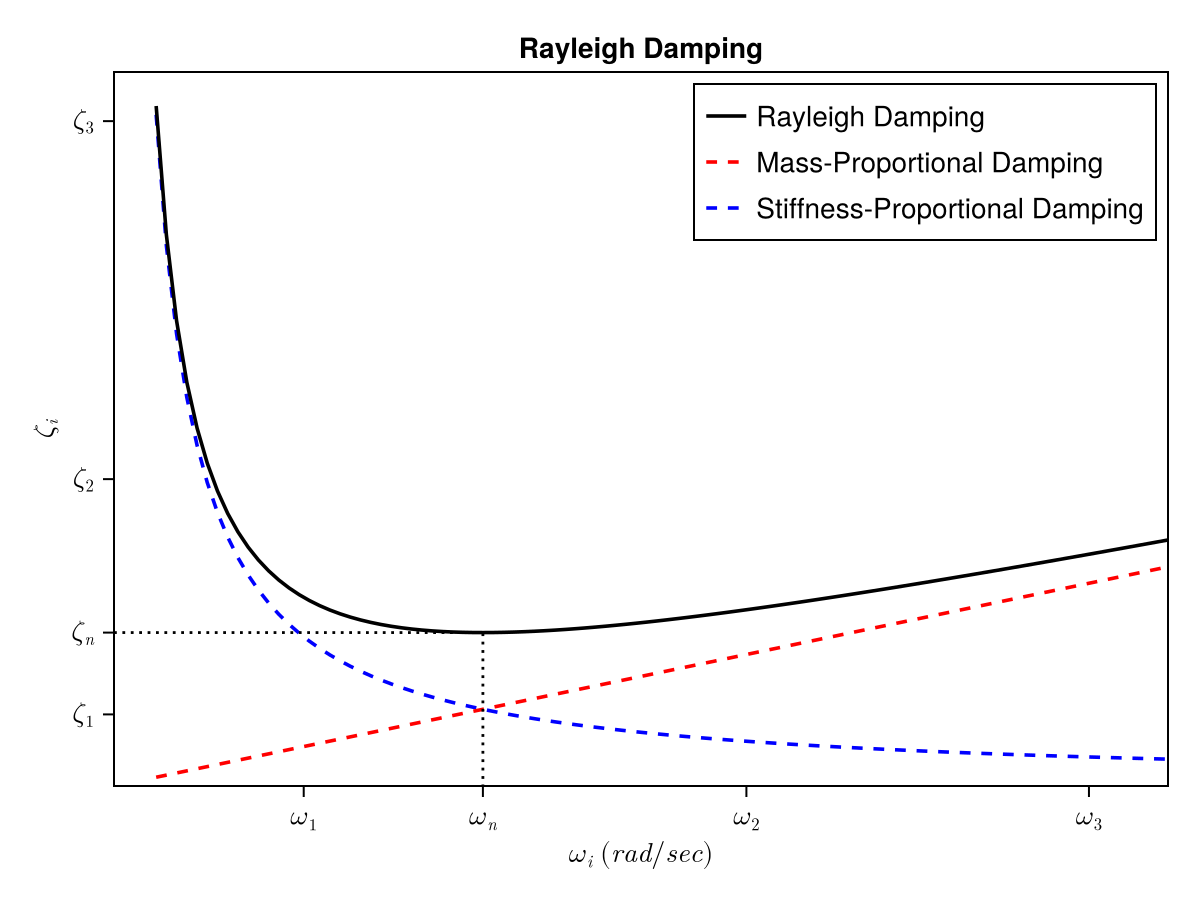
\includegraphics[width=0.94	\linewidth]{figures/fragility/rayleigh-damping.png}
	\caption{Μητρωική Απόσβεση Rayleigh}
	\label{fig:rayl}
\end{figure}

Για εφαρμογή απόσβεσης Rayleigh στο FLAC, επιλέγεται μία κεντρική συχνότητα $f_n$ (η ιδιοσυχνότητα $\omega_n$ υπολογίζεται εσωτερικά) και ο αντίστοιχος ιδιομορφικός λόγος απόσβεσης.

Η απόσβεση των φυσικών ιδιοσυχνοτήτων είναι βασικός λόγος χρήσης της απόσβεσης Rayleigh, έτσι εφαρμόζεται σε κάθε ζώνη των ακόλουθων αναλύσεων για την ομαλοποίηση των αποτελεσμάτων. Η μη-γραμμική συμπεριφορά των εδαφών όμως, δεν μπορεί να εκφραστεί απλώς από μία ενιαία απόσβεση που εφαρμόζεται παντού ίσα. Έτσι υπεισέρχεται στην εξίσωση η έννοια της υστερητικής απόσβεσης.

Η υστερητική απόσβεση ΑΑΑΑΑΑΑΑΑΑ

\begin{equation}
	V_s = \sqrt{\frac{G}{\rho}}
	\label{eq:vs}
\end{equation}

%Πρέπει να συνεχίσω με G-γ-D, υπάρχουν πολλά για να γράψω, αλλά πρέπει να καταλάβω λίγο καλύτερα τι παίζει με την απόσβεση, μόλις το πιάσω θα τα συμπληρώσω όλα.

%\subsection{Αλληλεπίδραση Εδάφους-Κατασκευής}
%%SSI
%Η αλληλεπίδραση εδάφους-κατασκευής (soil-structure interaction, SSI) συντελεί ένα κεντρικό θέμα %μελέτης για κάθε κατασκευή, καθώς όλες οι κατασκευές εδράζονται με κάποιον τρόπο στο έδαφος.%

%Συνηθέστερα σε στατικές αναλύσεις κτηρίων, ακολουθείται ο συλλογισμός ότι η κατασκευή εδράζεται σε πακτώσεις, και ύστερα γίνεται η επίλυση. Μία τέτοια παραδοχή όμως, μπορεί να ικανοποιεί αρχικά την στατική μελέτη, αλλά αγνοεί ένα βασικό στοιχείο του εδάφους: πως είναι και το ίδιο εύκαμπτο. Επομένως η προσομοίωση αυτή, συχνά αγνοεί την ευκαμψία του εδάφους, σφάλοντας σημαντικά στην συμπεριφορά των θεμελίων αλλά και στα εκτιμόμενα μεγέθη της κατασκευής.



\subsection{Λόγος Ευκαμψίας}
% Εξίσωση F
Όπως έχει ήδη αναφερθεί, οι σήραγγες σε αντίθεση με τις κοινές κατασκευές εξαρτόνται προτίστως από το περιβάλλον έδαφος και λιγότερο από τα χαρακτηριστικά της ίδιας κατασκευής.

Επομένως, ένα βασικό στοιχείο χαρακτηρισμού των σηράγγων είναι η ευκαμψία αυτής. Μία σήραγγα μπορεί να τοποθετηθεί σε δύο ακραίες κατηγορίες, χαρακτηριζόμενη ως εύκμαπτη και ως άκαμπτη.

Μία εύκαμπτη σήραγγα, δηλαδή μία σήραγγα απείρως πιο εύκαμπτη σε σχέση με το περιβάλλον έδαφος, της οποίας η επανακατανομή τάσεων και το παραμορφωμένο σχήμα δεν αναπτύσσει σημαντικές ροπές στην στήριξη της. Μία τέτοια διατομή εξαρτάται αποκλειστικά από τις κινήσεις του εδάφους και η δομική της συμπεριφορά περιγράφεται σε επίπεδο παραμορφώσεων.

Αντίθετα, μία άκαμπτη σήραγγα είναι εκείνη η οποία παραμορφώνεται ελάχιστα υπό των εδαφικών φορτίων και επομένως τα παραλαμβάνει. Τέτοιες σήραγγες εμφανίζουν σχεδόν μηδενική αλληλεπίδραση εδάφους κατασκευής. Οποιαδήποτε από τις δύο ακραίες περιπτώσεις είναι αδύνατον να εμφανιστούν σε πραγματικές συνθήκες πεδίου, επομένως μία μέση τιμή πρέπει να οριστεί και να αξιοποιηθεί.

Φυσικά, η ευκαμψία μίας σήραγγας δεν μπορεί να οριστεί αυτοτελώς, αλλά πάντα πρέπει να περιγραφεί σε σχέση με τις εδαφικές συνθήκες. Έτσι έχει αναπτυχθεί ο λόγος ευκαμψίας.

Γενικότερα, η δυσκαμψία της σήραγγας περιγράφεται με δύο τρόπους. Αφενός μπορεί να περιγραφεί σε σχέση με την δυστένεια της, υπολογίζοντας μία ομοιόμορφη πίεση που θα προκαλούσε μοναδιαία διαμετρική παραμόρφωση χωρίς μεταβολή του σχήματος. Αφετέρου, και σε σχέση με την κάμψη της, ως μέτρηση της ανομοιόμορφης πίεσης που προκαλεί μοναδιαία διαμετρική μεταβολή της σήραγγας με αλλαγή του σχήματος της σε έλλειψης.

Ο λόγος ευκαμψίας υπολογίζεται σε καθαρή διάτμηση, από την αντίσταση της διατομής σε διαμετρική παραμόρφωση. Η Εξίσωση \ref{eq:dstrain} περιγράφει την ανηγμένη διαμετρική παραμόρφωση κατά την οβαλοποίηση.

\begin{equation}
	\frac{\Delta D}{D} = \frac{p}{E_s}(1+v)
	\label{eq:dstrain}
\end{equation}

Οι εδαφικές πιέσεις που ωθούν κυκλική διατομή σε τέτοια αλλαγή σχήματος, εκφράζονται σε σχέση με την αδράνεια λεπτού δακτυλίου από την Εξίσωση \ref{eq:dstrain2}.

\begin{equation}
	\frac{\Delta D}{D} = \frac{p\cdot R^3}{6E_l\,I_l}
	\label{eq:dstrain2}
\end{equation}

Αντικαθιστώντας τον όρο $E_l\,I_l$ με $E_l\,I_l/(1-v_l^2)$ έτσι ώστε να συνυπολογίζεται η κατάσταση επίπεδης παραμόρφωσης, και διαιρώντας με την Εξίσωση \ref{eq:dstrain}, προκύπτει η σχέση υπολογισμού του λόγου ευκαμψίας με την μορφή της Εξίσωσης \ref{eq:flex} \parencite{Peck}.

\begin{equation}
	F = \frac{E_s(1-v_l^2)R^3}{6E_l I_l(1+v)}
	\label{eq:flex}
\end{equation}

Όπου, στην Εξίσωση \ref{eq:flex} με $l$ υποδεικνύονται τα μεγέθη που αφορούν στα τοιχώματα της σήραγγας, ενώ με $s$ τα μεγέθη του περιβάλλοντος εδάφους.

Η συλλογιστική και υπολογιστική πορεία που οδηγεί στο συμπέρασμα του λόγου ευκαμψίας, είναι και η ίδια που επιτρέπει την εύκολη επιλογή σε EDPs. Καθώς θεωρείται ότι τα διατμητικά κύματα προκαλούν τυπικώς καθαρή διάτμηση στην διατομή, επομένως οι εύκαμπτες σήραγγες που υπόκεινται σε καθαρή διάτμηση θα παρουσιάζουν οβαλοποίηση και η διατμητική παραμόρφωση του εδάφους θα έχει ισχυρή συσχέτιση με την ανηγμένη διαμετρική παραμόρφωση των σηράγγων.

Έτσι, οι σήραγγες μπορούν να κατηγοριοποιηθούν σύμφωνα με τον λόγο ευκαμψίας σε στατικές συνθήκες, πρωτού πραγματοποιηθούν οι αριθμητικές αναλύσεις. Από τα αποτελέσματα των αναλύεσων, μπορεί να συγκριθεί η συσχέτιση των EDPs, δηλαδή της διαμετρικής παραμόρφωσης και ροπής, με τα μεγέθη έντασης (εμμέσως λοιπόν και με την διατμητική παραμόρφωση του εδάφους) ώστε να διαπιστωθεί το μέγεθος αντίστασης των σηράγγων στο έδαφος.


\subsection{Φάσμα Πλάτους Fourier}
% Κάποιες εξισώσεις ίσως, αλλιώς γενική περιγραφή
Στις προηγούμενες ενότητες, έχει γίνει αναφορά στο συχνοτικό περιεχόμενο των σεισμικών κινήσεων και, ενώ η Επικινδυνότητα χαρακτηρίζεται συνήθως από μεγέθη αποκρίσεων, οι σημαντικές συχνότητες μίας σεισμικής κίνησης αποτελούν κρίσιμη παράμετρο για την επιρροή που έχει στις κατασκευές.

Είναι γνωστό από την δυναμική των συνεχών μέσων, ότι ένα σώμα που υπόκεινται σε εξαναγκασμένη ταλάντωση παρουσιάζει ενίσχυση της παρατηρούμενης απόκρισεις όταν η συχνότητα της διέγερσης προσεγγίζει συγκεκριμένες συχνότητες. Το συγκεκριμένο φαινόμενο ονομάζεται συντονισμός, και οι συχνότητες στις οποίες εμφανίζεται αποκαλούνται οι ιδιοσυχνότητες του σώματος όπως καθορίζονται από τα χαρακτηριστικά του, κυρίως την μάζα και την δυσκαμψία \parencite{Clough}. % Άναφορά Clough-Penzien

Είναι σαφές λοιπόν ότι ένα σεισμικό γεγονός δεν αρκεί να χαρακτηριστεί μονάχα από ένα μέγεθος έντασης, αλλά απαιτείται και το συχνοτικό περιεχόμενο για μία πιο πλήρη εικόνα. Επομένως, έχει αναπτυχθεί μία μεθοδολογία η οποία επιτρέπει την συχνοτική ανάλυση μίας χρονοϊστορίας. Αυτή η μέθοδος ονομάζεται μετασχηματισμός Fourier.

\begin{figure}[h]
	\centering
	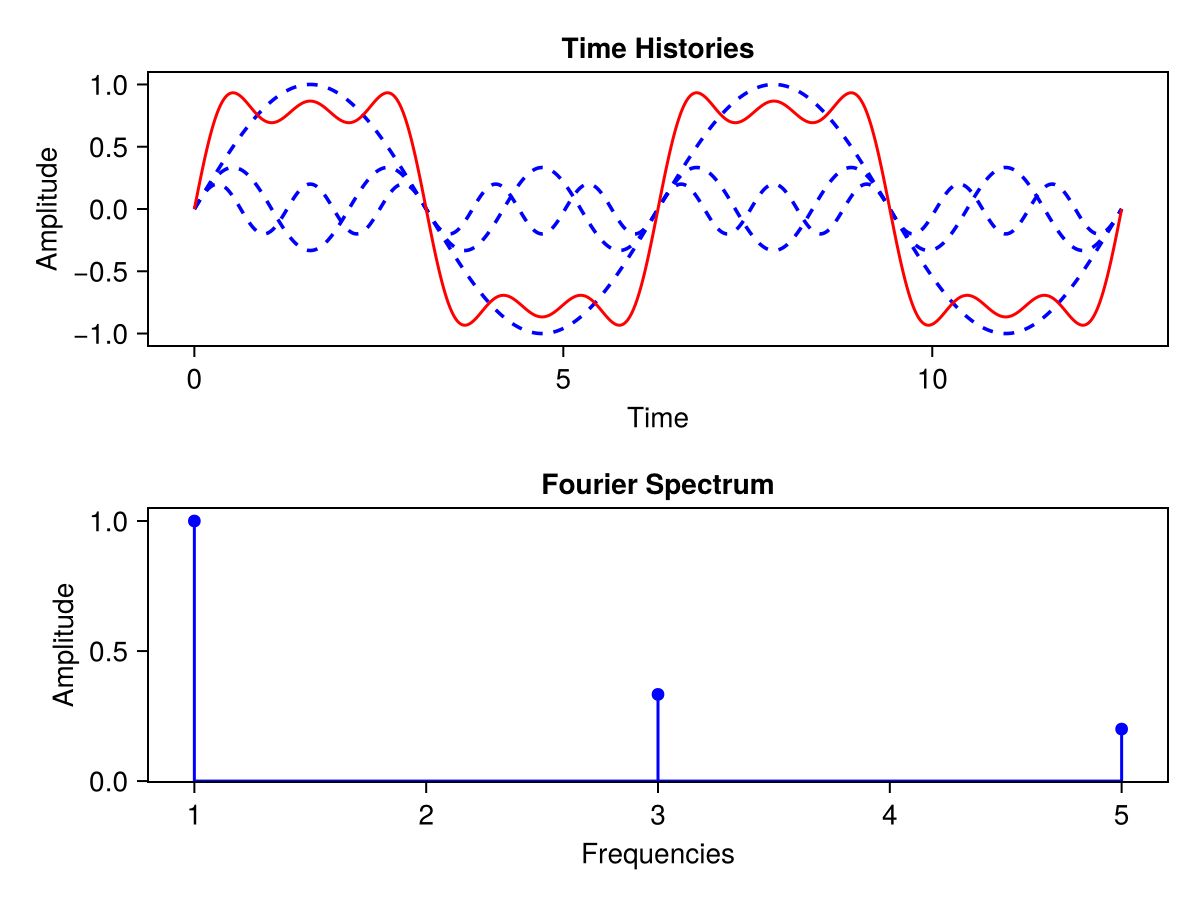
\includegraphics[width=0.94\linewidth]{figures/fragility/FAS.png}
	\caption{Παράδειγμα Μετασχηματισμού Fourier}
	\label{fig:four}
\end{figure}

Το θεώρημα του Fourier θέτει πως οποιαδήποτε συνάρτηση μπορεί να εκφραστεί από ένα άθροισμα ημιτόνων ή συνημιτόνων με συγκεκριμένο πλάτος και γωνία φάσης για κάθε συχνότητα. Συνεπώς, για κάθε συνάρτηση μπορεί να αποτυπωθεί το πλάτος ή η γωνία φάσης σε σχέση με την αντίστοιχη συχνότητα, αποτυπώνοντας το συχνοτικό περιεχόμενο \parencite{Fourier}, έχοντας ως γενική σχέση μετασχηματισμού της συνάρτησης συσχετισμού απόκρισης με τον χρόνο σε ιδιοσυχνότητες την Εξίσωση \ref{eq:fourier}.

\begin{equation}
	X(\omega) = \int_{-\infty}^{+\infty} x(t)e^{-j\omega t}dt
	\label{eq:fourier}
\end{equation}

Μία κλασική περίπτωση που χρησιμοποιείται συχνά για την περιγραφή της μεθόδου Fourier είναι η κατασκευή ενός τετραγωνικού παλμού ως άθροισμα ημιτόνων όπως ορίζεται από την Εξίσωση \ref{eq:square}.

\begin{equation}
	y = \sum_{k=0}^\infty \frac{\sin{(2k+1)\pi\,x}}{2k+1}
	\label{eq:square}
\end{equation}

Στο Σχήμα \ref{fig:four} απεικονίζεται τα τρία πρώτα ημίτονα της Εξίσωσης \ref{eq:square} με το άθροισμα αυτών καθώς και το αντίστοιχο φάσμα Fourier. Το άθροισμα άπειρων ημιτόνων επιτρέπει την ακριβή κατασκευή τετραγωνικού παλμού.

%Πρώτα μέθοδος Fourier και τέτοια

\begin{equation}
	F(t) = \sum_{n=-\infty}^{+\infty}\delta (t-nT)
	\label{eq:per-comp}
\end{equation}

 Στην περίπτωση περιοδικών συναρτήσεων, όπως είναι ένα σεισμικό κύμα, τότε αυτή η συνάρτηση πορεί να εκφραστεί σύμφωνα με την δέλτα συνάρτηση Ντιράκ όπως γίνεται στην Εξίσωση \ref{eq:per-comp}  \parencite{Racheva}. Η συγκεκριμένη σχέση αναπαρίσταται καλύτερα από την ταυτότητα του Euler στην Εξίσωση \ref{eq:per-four}.
 
\begin{equation}
	F(t) = \frac{1}{T}\sum_{n=-\infty}^{+\infty}e^{i2\pi nt/T}
	\label{eq:per-four}
\end{equation}

Η σημασία των φασμάτων διαφαίνεται εύκολα, η μεγάλη δυσκολία όμως ξεχωρίζει στις μεθόδους εκτέλεσης του μετασχηματισμού, με συνηθέστερη την χρήση του ταχέως μετασχηματισμού Fourier (Fast Fourier Transform, FFT).

Μία θεωρητική προσέγγιση του μετασχηματισμού Fourier μπορεί να πραγματοποιηθεί για κάποια γνωστή συνάρτηση, αλλά στην μηχανική πράξη, οι καταγραφές κυμάτων δεν αποτελούν γνωστές συναρτήσεις αλλά διακριτοποιημένες και δειγματόληπτες τιμές. Η κατανόηση της σεισμικής μηχανικής δεν έχει εξελιχθεί σε τέτοιο βαθμό ώστε να μπορούν σύνθετα κύματα να περιγράφονται από συναρτήσεις, επομένως οι επεξεργασμένες σεισμικές καταγραφές αποτελούν τον καλύτερο τρόπο χρήσης και αναπαραγωγής χρονοϊστοριών. Για αυτό τον λόγο είναι απαραίτητη η χρήση της FFT, έτσι ώστε να παραχθεί το φάσμα της αντίστοιχης καταγραφής.

Η FFT βασίζεται στον διακριτό μετασχηματισμό Fourier (Discrete Fourier Transform, DFT) όπου το συνεχές ολοκλήρωμα αντικαθίσταται με το αντίστοιχο άθροισμα διακριτών τιμών όπως στην Εξίσωση \ref{eq:dft} σε προσαρμογή της Εξίσωσης \ref{eq:fourier} \parencite{Smith}.

\begin{equation}
	X(\omega_k) \triangleq \sum_{n=0}^{N-1} x(t_n) e^{-j\omega_kt_n}
	\label{eq:dft}
\end{equation}

Με την μετασχηματισμένη Εξίσωση, μία μεγάλη διαφορά στις παραμέτρους είναι το γεγονός ότι ο χρόνος παύει να αντιμετωπίζεται συνεχώς αλλά ορίζεται το χρονικό ισοδιάστημα δειγματοληψίας. Κατά αυτή την έννοια κιόλας, ο άριθμός των ξεχωριστών ημιτόνων που υπολογίζονται είναι ίσος με τον αριθμό δειγμάτων του κύματος.

Ακόμα και ο διακριτός υπολογισμός των φασμάτων δύναται να φέρει υψηλό υπολογιστικό φορτίο και επομένως να απαιτούν πολύ διάρκεια επίλυσης καθώς ο γραμμικός υπολογισμός απαιτεί $N^2$ πράξεις, έτσι στην αρχή του προηγούμενου αιώνα αναπτύχθηκε μία μέθοδος υπολογισμού του διακριτού φάσματος σε λιγότερο από $2N\log_2 N$ πράξεις και χρησιμοποιώντας λίγη μνήμη \parencite{Cooley}. 

Αυτή η μέθοδος στην πορεία διαμορφώθηκε στην FFT. Εν ολίγοις στην μέθοδο, αξιοποιείται η ορθογωνικότητα του πίνακα διακριτών δειγμάτων έτσι ώστε να επιλυθεί το ένα μέρος του μόνο, μειώνοντας δραματικά τους υπολογισμούς \parencite{Brigham}.

%\subsection{Response Spectra}
\subsection{Συνάρτηση Μεταφοράς}
\label{sbs:tf}
% Εφόσον ορίζεται το FAS, ορίζονται εύκολα οι TF
% Λόγος FAS
Έχοντας ορίσει τα φάσματα πλάτους Fourier, σπουδαία σημασία για την μετάδοση των σεισμικών κυμάτων στο έδαφος είναι η συνάρτηση μεταφοράς.

Ένα σεισμικό κύμα που διαδίδεται κατακόρυφα μέσα από μία εδαφική στήλη, μπορεί να συναντήσει μία σύνθετη στρωματογραφία με στρώματα διαφορετικής δυσκαμψία, πυκνότητας ή άλλων παραμέτρων, προκαλώντας το σεισμικό κύμα να μεταβληθεί ως προς το πλάτος και το συχνοτικό του περιεχόμενο από τα διάφορα φαινόμενα διάθλασης, ανάκλασης και σκέδασης. Επιπροσθέτως, η μη-γραμμική συμπεριφορά του εδάφους, όπως περιγράφεται και στην Υποενότητα \ref{sbs:damping}, οδηγεί το έδαφος να ανταποκρίνεται με διαφορετικό τρόπο για διαφορετικό βαθμό παραμόρφωσης.

Έτσι, η κατακόρυφη διάδοση ενός διατμητικού κύματος σε μία συγκεκριμένη στήλη, μπορεί να υποστεί πολύ διαφορετική μεταβλή σε μία άλλη στήλη, καθώς και ένα διαφορετικό κύμα στην ίδια στήλη.

Αυτά τα φαινόμενα λοιπόν, μπορούν να περιγραφούν άριστα με μία συνάρτηση μεταφοράς. Η συναρτήσεις μεταφοράς ορίζονται συνήθως ως ο λόγος δύο φασμάτων πλάτους Fourier όπου το ένα από τα δύο προκύπτει εμμέσως από το άλλο έτσι ώστε να αποτυπώνεται η ενίσχυση που συμβαίνει σε κάθε συχνότητα. Συνήθως, οι συναρτήσεις μεταφοράς λαμβάνονται σε μία εδαφική στήλη ως η ενίσχυση της επιτάχυνσης από το βραχώδες υπόβαθρο ως την επιφάνεια ή ως ο λόγος των οριζόντιων προς τις κατακόρυφες επιταχύνσεις ενός σημείου \parencite{Garcia}.

Στην παρούσα εργασία οι συναρτήσεις μεταφοράς λαμβάνονται για την επιβεβαίωση αριθμητικών αναλύσεων, συγκρίνοντας με θεωρητικές λύσεις προβλημάτων.

\begin{equation}
	T_0 = \frac{4H}{V}
	\label{eq:T0}
\end{equation}

Ως παράδειγμα, για εδαφική στήλη δεδομένης ταχύτητας διάδοσης διατμητικών κυμάτων, η συνάρτηση μεταφοράς μπορεί να βαθμονομηθεί σε σχέση με τις αναλυτικές τιμές ιδιοπεριόδων του εδάφους όπως υπολογίζεται από την Εξίσωση \ref{eq:T0} \parencite{Dobry}.

Μία πολύ σημαντική λεπτομέρεια για τις συναρτήσεις μεταφοράς, είναι ότι στην πράξη η κάθε μία είναι μοναδική σε σχέση με την χρονοϊστορία που την παράγει. Λόγω της υστερητικής απόσβεσης, μία ανίσχυρη εδαφική κίνηση θα είναι κοντά στην ελαστική συμπεριφορά του εδάφους και θα είναι πιο προβλέψιμη, ενώ μία πολύ ισχυρή δύναται να προκαλέσει πολύ έντονη μη-γραμμική συμπεριφορά και σχετικά απρόβλεπτα αποτελέσματα στο έδαφος.

\section{Βαθμονόμηση Αριθμητικού Μοντέλου}
%Εδώ θα γίνει αρχικά η αναφορά στην βαθμονόμηση, μία γενική περιγραφή για το 

Έχοντας ορίσει τις βασικές έννοιες για την πραγματοποίηση αριθμητικών αναλύσεων και την εξαγωγή αποτελεσμάτων, είναι καιρός να καταστρωθούν τα αριθμητικά μοντέλα.

Πρωτού όμως εκτελεστούν οι πλήρεις δυναμικές αναλύσεις, πρέπει να επιβεβαιωθεί η εύρυθμη λειτουργία του προγράμματος πεπερασμένων διαφορών και των αριθμητικών προσομοιωμάτων.

Για να επιτευχθεί αυτό, γίνεται σύγκριση μεταξύ θεωρητικών λύσεων και αποτελεσμάτων αριθμητικών αναλύσεων.

\subsection{Περιγραφή Μεθόδου}
Ο τρόπος που βαθμονομείται ένα εδαφικό προσομοίωμα πεπερασμένων διαφορών σε δυναμικές σεισμικές δράσεις βασίζεται συνήθως σε μία σαφή σειρά βημάτων.

Πρώτα επιλέγεται το εργαλείο προς χρήση, που χρειάζεται να βαθμονομηθεί και το αντίστοιχο εργαλείο υπολογισμού της μονοδιάστατης διάδοσης κυμάτων σε εδαφική στήλη, βασιζόμενο σε θεωρητικές λύσεις. Εν προκειμένω χρησιμοποιείται ως πρόγραμματα το FLAC για ανάλυση πεπερασμένων διαφορών, και το Strata για μονοδιάστατη σεισμική ανάλυση εδαφικής στήλης.

Στην συνέχεια, εισαγάγοντας την ίδια σεισμική χρονοϊστορία, σε δύο ισοδύναμα προσομοιώματα, στο κάθε εργαλείο συγκρίνονται οι λύσεις ώστε να αποφανθεί η σύγκλιση των.

Όπως αναφέρθηκε και στην Υποενότητα \ref{sbs:tf}, η βασική σύγκριση που γίνεται είναι η συνάρτηση μεταφοράς του αριθμητικού προσομοιώματος, με αυτή του Strata, και όλες μαζί με τις θεωρητικές συχνότητες κατά Dobry.

\subsection{Προσομοίωμα}
Η βαθμονόμηση του μοντέλου πραγματοποιείται σταδιακά ώστε να επιτευχθεί η μέγιστη δυνατή ποιότητα των αποτελεσμάτων.

Πρώτα κατασκευάζεται το ελαστικό μοντέλο, στο οποίο αναμένεται απόλυτη σύγκλιση μεταξύ των προγραμμάτων καθώς και το Strata και οι υπόλοιπες άναλυτικές λύσεις βασίζονται σε συνεχή και ελαστική συμπεριφορά του υλικού.

Στην συνέχεια, επιλύεται η περίπτωση της μη-γραμμικής συμπεριφοράς του εδάφους, όπως θα είναι και στα τελικά προσομοιώματα. Όταν το έδαφος λειτουργεί μη-γραμμικά, η διάδοση των διατμητικών κυμάτων διαφέρει σημαντικά από την θεωρητική καθώς οι διατμητικές παραμορφώσεις του εδάφους ενεργοποιούν την υστερητική του συμπεριφορά μεταβάλλοντας το συχνοτικό περιεχόμενο και τα πλάτη της κίνησης. Η μείωση του μέτρου δυσκαμψίας με την παραμόρφωση προκαλεί μείωση της ταχύτητας διάδοσης διατμητικών κυμάτων κατά την Εξίσωση \ref{eq:vs} οπότε και η συχνότητες συντονισμού αναμένεται να μειωθούν κατά την Εξίσωση \ref{eq:T0}.

Το FLAC μπορεί να εκτελέσει πλήρεις μη-γραμμικές αναλύσεις, αλλά δεν ισχύει το ίδιο για το Strata. Αυτό βασίζεται στην ισοδύναμη-γραμμική μέθοδο κατά την οποία το υλικό συμπεριφέρεται γραμμικά, επιλέγοντας αυτόματα και εκ προοιμίου το μέτρο διάτμησης και την απόσβεση εισαγάγοντας την αναμενόμενη διατμητική παραμόρφωση που θα προκαλέσει η εδαφική κίνηση ως παράμετρο στις καμπύλες G-γ-D. Κατά αυτόν τον τρόπο η μέθοδος δεν ανταποκρίνεται στις πραγματικές συνθήκες, αλλά μπορεί να προσεγγίσει με έναν θεωρητικό τρόπο τα αποτελέσματα.

Η τελευταία ανάλυση που πραγματοποιείται για την βαθμονόμηση είναι αυτή του πολυστρωματικού εδάφους, τριών στρώσεων. Μία υποπερίπτωση της μη-γραμμικής συμπεριφοράς, διατηρώντας ίδια την μέση ταχύτητα διάδοσης διατμητικών κυμάτων για την εδαφική στήλη, αλλά αυξάνοντας βαθμιαία την δυστμησία του εδάφους με κάθε βαθύτερη στρώση.

Η συμπεριφορά των δύο τελευταίων αναλύσεων πρέπει να είναι παρόμοια, ενώ οι πρώτες προκύπτουσες συχνότητες συντονισμού πρέπει να συγκλίνουν μεταξύ των δύο μεθόδων. Το ίδιο δεν ισχύει απαραίτητα και για τα πλάτη απόκρισης, διότι οι θεωρητικές λύσεις αναμένουν συνήθως μείωση της απόκρισης σε μεγαλύτερες συχνότητες όταν οι υπερκείμενες στρώσεις είναι πιο εύκαμπτες, ενώ στην πράξη δεν ισχύει πάντα το ίδιο.

Το ίδιο το προσομοίωμα πρόκειται για μία εδαφική στήλη ύψους 51.5 και πλάτους 5 μέτρων, αποτελούμενη από στοιχεία διαστάσεων $0.5m\times 0.5m$. Κανονικά η εδαφική στήλη στο προσομοίωμα πρέπει να έχει πλάτος ίσο με ένα στοιχείο για να αποφεύγονται τα φαινόμενα διάθλασης και ανάκλασης που συνοδεύουν την δισδιάστατη ανάλυση, αλλά στην προκειμένη περίπτωση δόθηκε ένα μικρό πλάτος για να βεβαιωθεί κατά το μέγιστο δυνατόν η πλήρης λειτουργίας του εδάφους.

Η χρονοϊστορία εισαγάγεται στην βάση του προσομοιώματος, σε θεωρητικό βραχώδες ελαστικό και απείρως στιβαρό. Έτσι η βάση του προσομοιώματος δεσμεύεται σε κίνηση μόνο κατά τον κατακόρυφο και τα πλευρικά όρια δεσμεύονται με εννιαία οριζόντια μετατόπιση σε κάθε κόμβο ίδιας τεταγμένης (Tie Constraints).

Το προσομοίωμα έρχεται πρώτα σε ελαστική ισορροπία υπό το ίδιο του βάρος και έπειτα χρησιμοποιείται το καταστατικό του μοντέλο για την πλήρη δυναμική ανάλυση. Στην δυναμική ανάλυση, χρησιμοποιείται απόσβεση Rayleigh για κάθε προσομοίωμα, και σιγμοειδείς G-γ-D για κάθε μη-γραμμική στρώση εδάφους, όπου η κάθε σιγμοειδής εισαγάγεται σε σχέση με τρεις παραμέτρους από την επιλογή sig3 του FLAC.

%για την απόσβεση Rayleigh, τάδε κρίσιμης απόσβεσης $\zeta_{min}$ στην κρίσιμη συχνότητα $\omega_n$ κατά το Σχήμα \ref{fig:rayl}.


\begin{figure}[h]
	\centering
	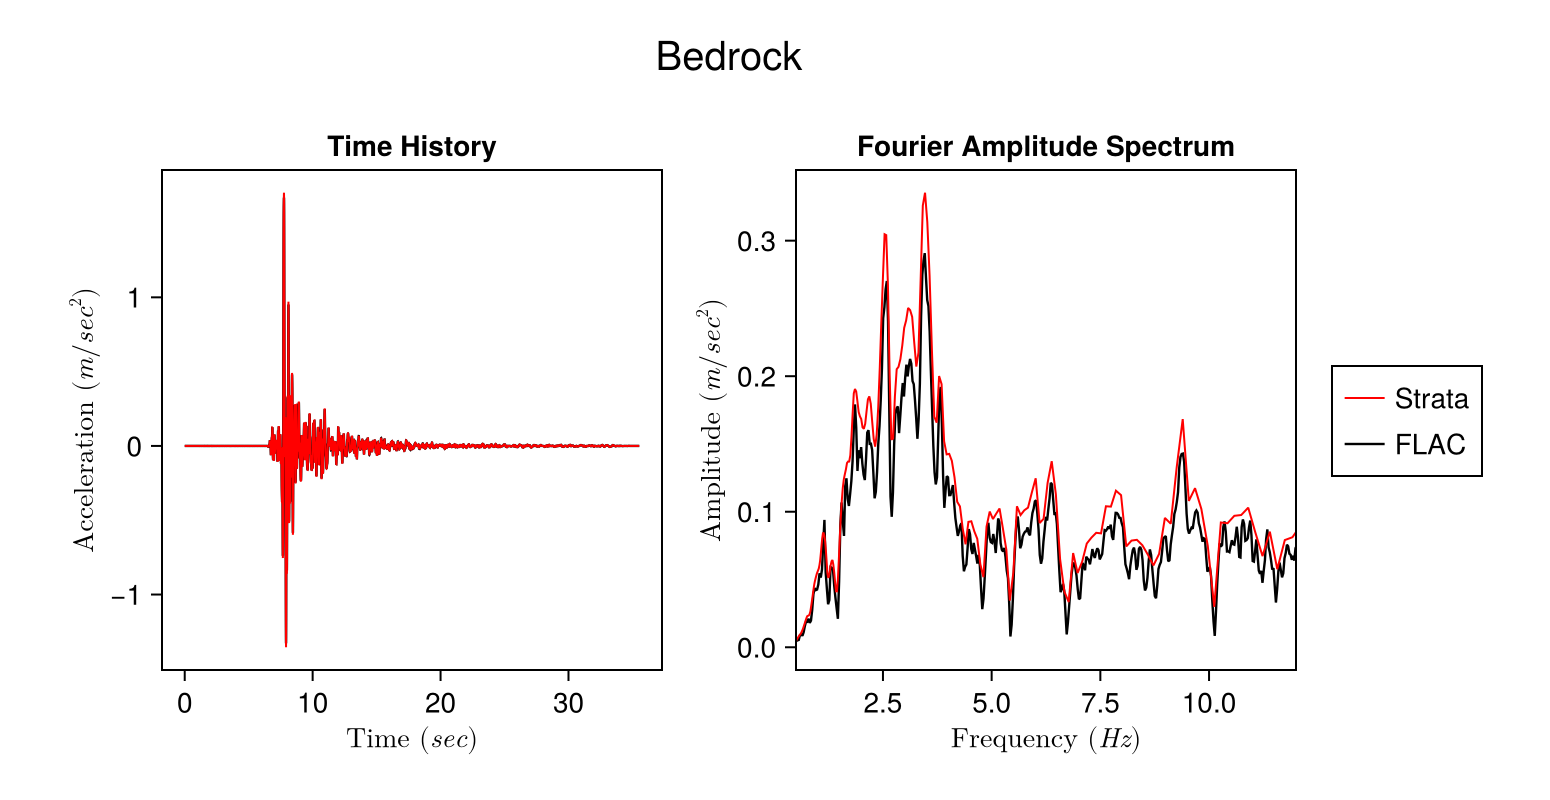
\includegraphics[width=\linewidth]{figures/fragility/Base.png}
	\caption{Εισαγώμενη Χρονοϊστορία Βραχώδους Υποβάθρου}
	\label{fig:base-th}
\end{figure}

Το καταστατικό μοντέλο του υλικού είναι αρχικά ελαστικό και έπειτα Mohr-Coulomb, με μέτρο διάτμησης $G = 180\;MPa$ που αντιστοιχεί σε ταχύτητα $V_s \approx 300\;m/sec$.

Από την ταχύτητα και το πλάτος των στοιχείων προκύπτει ότι το ελάχιστο μήκος κύματος είναι $5\;m$ που αντιστοιχεί σε μέγιστη συχνότητα $f \approx 63 Hz$. Αυτή η συχνότητα υπερβαίνει κατά πολύ την τάξη μεγέθους που ενδιαφέρει στα σεισμικά κύματα, επομένως το κριτήριο πληροίται με ευκολία.

Παρά την θεωρία, στις υψηλές συχνότητες η τιμή εισαγωγής μπορεί να είναι σχεδόν μηδενική αλλά για κάποιον λόγο η επιφανειακή απόκριση να λαμβάνει τιμές κάποιας μικρής τάξης μεγέθους, δίνοντας στο πηλίκο πολύ μεγάλη ενίσχυση φαινομενικά. Το ίδιο μπορεί να συμβαίνει και στις πολύ χαμηλές συχνότητες, όπου η ενίσχυση πρέπει να είναι μοναδιαία καθώς η φόρτιση θεωρείται ψευδοστατική.

Λόγω αριθμητικών σφαλμάτων μία τέτοια αποτύπωση μπορεί να μην είναι δυνατή. Έτσι όλα τα φάσματα πλάτους Fourier και οι συναρτήσεις μεταφοράς απεικονίζονται στα όρια συχνοτήτων $f = 0.5-12\;Hz$ όπου είναι και οι πιο χρήσιμες συχνότητες στην τεχνική σεισμολογία.

\subsection{Χρονοϊστορία}
Όπως αναφέρθηκε ήδη, οι συναρτήσεις μεταφοράς διαμορφώνονται σημαντικά από την χρονοϊστορία που τις προκαλεί. Έτσι, η κατάλληλη επιλογή για την χρονοϊστορία είναι ιδιαιτέρως κρίσιμη.

Οι τελικές αναλύσεις που πραγματοποιούνται στις σήραγγες του μετρό Θεσσαλονίκης αξιοποιούν ένα σύνολο από σεισμικές καταγραφές, κειμενόμενες από πολύ ασθενείς σε εξαιρετικά ισχυρές έτσι ώστε η στατιστική κατανομή που εφαρμόζεται να προσεγγίζει κατά το βέλτιστο την πραγματικότητα. Άρα και το έδαφος, σε κάποιες χρονοϊστορίες θα συμπεριφέρεται σχεδόν ελαστικά ενώ σε άλλες η πλαστικοποίηση θα προσδίδει απρόβλεπτα αποτελέσματα.

Εξού και η επιλογή χρονοϊστορίας θεωρείται ότι είναι καλό να προσεγγίζει την απρόβλεπτη φύση του προβλήματος, ξεπερνώντας την ελαστική συμπεριφορά, ενώ όμως διατηρείται σε επίπεδα όπου μία θεωρητική σύγκριση να είναι δυνατή. Για αυτόν τον λόγο επιλέχθηκε χρονοϊστορία μέγιστης εδαφικής επιτάχυνσης ίσης με $0.167g$ όπως απεικονίζεται στο Σχήμα \ref{fig:base-th}.

Θα μπορούσε να εκτελεστούν ένα σύνολο από αναλύσεις για χρονοϊστορίας πληθώρας μεγεθών έντασης, αλλά κάτι τέτοιο θεωρήθηκε περιττό για τις ανάγκες της παρούσας εργασίας.


Στο Σχήμα \ref{fig:base-th} απεικονίζεται η χρονοϊστορία και το αντίστοιχο φάσμα της, όπως εισήχθη στο FLAC και στο Strata αντίστοιχα. Η σύγκριση παρουσιάζεται διότι η χρονοϊστορία είναι μεν ίδια και στις δύο περιπτώσεις, αλλά το Strata πραγματοποιεί κάποιες ομαλοποιήσεις και διορθώσεις στις εισαγώμενες κινήσεις, προκαλώντας μικρές μεταβολές στις τιμές της.

Η αναφορά στην διαφοροποίηση γίνεται και για τον εξής λόγο. Το Strata μεταβάλλει την χρονοϊστορία με τέτοιον τρόπο έτσι ώστε τα αποτελέσματα της να έχουν αριθμό σημείων ίσο με κάποια δύναμη του δύο. Ο λόγος είναι ότι κάποιες μέθοδοι DFT δουλεύουν αποκλειστικά με τέτοιον αριθμό σημείων, ενώ γενικά είναι ταχύτερη. Το FLAC όμως απαιτεί όσο το δυνατόν πιο λεπτά διακριτοποιημένη την χρονοϊστορία, και δεν πραγματοποιεί τέτοια μεταβολή, έτσι τα δύο φάσματα έχουν κάποια αριθμητική απόκλιση στο πλάτος και στην λεπτομέρεια, ενώ η μορφή είναι κατά βάση ίδια.

\begin{figure}[h]
	\centering
	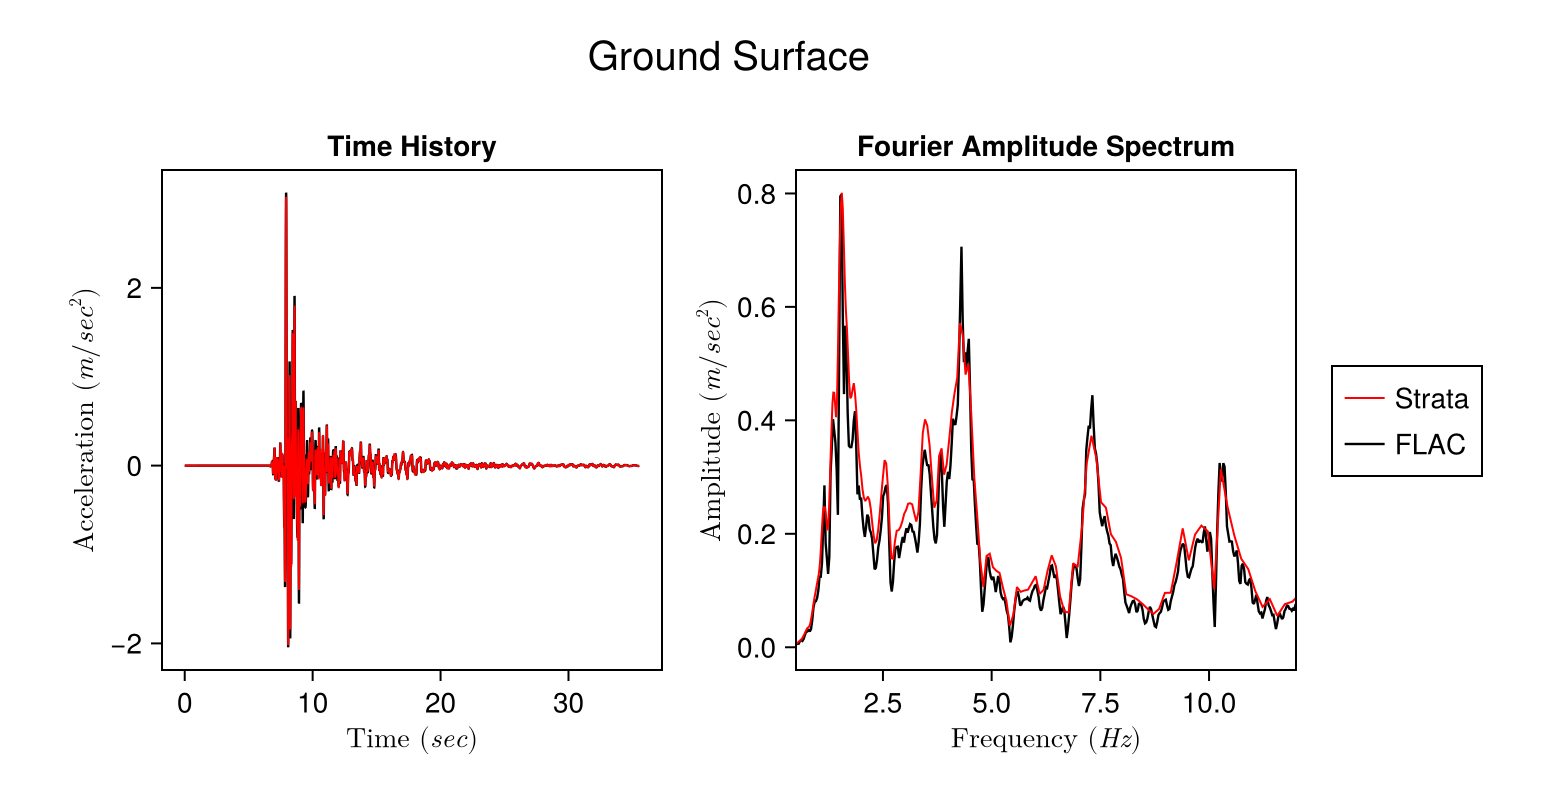
\includegraphics[width=\linewidth]{figures/fragility/Top-Elastic.png}
	\caption{Επιφανειακή Απόκριση Ελαστικής Ανάλυσης}
	\label{fig:el-sur}
\end{figure}

\subsection{Ελαστικό Μοντέλο}

Η πρώτη πραγματοποιούμενη ανάλυση είναι αυτή της ελαστικής περίπτωσης, στην οποία το καταστατικό μοντέλο της αριθμητικής ανάλυσης συμπεριφέρεται γραμμικά-ελαστικά και δεν χρησιμοποιείται υστερητική απόσβεση παρά μόνο μητρωική Rayleigh.

Εκτελώντας την ανάλυση, προκύπτει η επιφανειακή απόκριση και το αντίστοιχο φάσμα πλάτους Fourier κατά το Σχήμα \ref{fig:el-sur}

%Το ισοδύναμο-γραμμικό μοντέλο επιλέγει μία μέση απόσβεση και δυστμησία για όλη την διάρκεια φόρτισης, επομένως σε ισχυρές κινήσεις η απόσβεση θα είναι χαμηλή και το έδαφος πολύ στιβαρό, ενώ σε χαμηλές η απόσβεση θα είναι μεγάλη και το έδαφος πιο χαλαρό. Αυτό το φαινόμενο διαφαίνεται στο Σχήμα \ref{fig:el-sur}, καθώς η απόκριση στο Strata έχει μικρότερα πλάτη σε σχέση με το FLAC στα πιο υψηλά σημεία της χρονοϊστορίας, ενώ σε χρόνο μέσης έντασης οι δύο χρονοϊστορίες ταυτίζονται σχεδόν απόλυτα.

\begin{figure}[h]
	\centering
	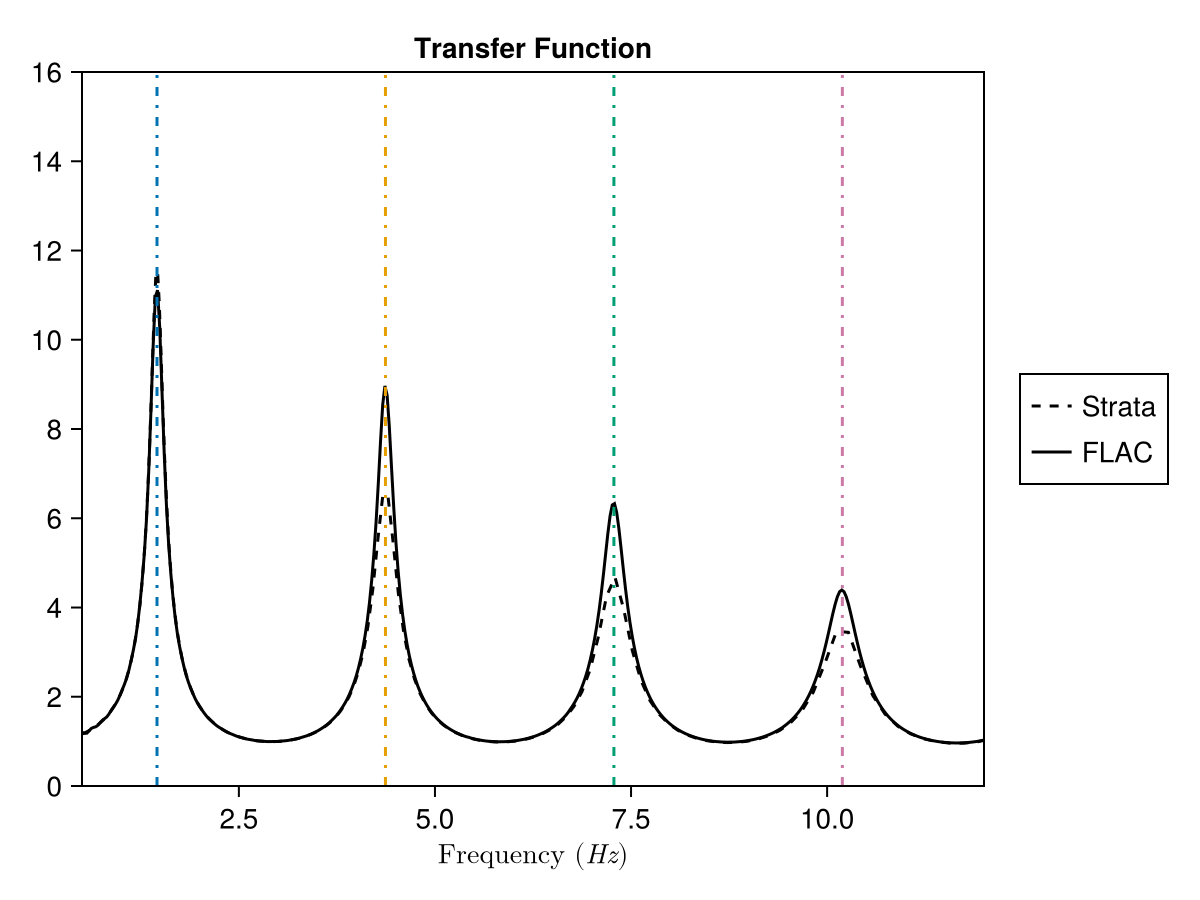
\includegraphics[width=0.8\linewidth]{figures/fragility/TF-Elastic.png}
	\caption{Συνάρτηση Μεταφοράς Ελαστικής Ανάλυσης}
	\label{fig:el-tf}
\end{figure}

Το φάσμα εισαγωγής έχει σχετικά ομοιόμορφο πλάτος, παρουσιάζοντας μεγαλύτερες τιμές περίπου στο εύρος συχνοτήτων $f=2-4\;Hz$ όπου είναι η ισχυρή εδαφική κίνηση. Αντίθετα, το φάσμα απόκρισης έχει πολύ σαφείς κορυφές, υποδεικνύοντας φαινόμενα συντονισμού σε αυτές τις συχνότητες.

Πράγματι από την συνάρτηση μεταφοράς του Σχήματος \ref{fig:el-tf}, οι συχνότητες του φάσματος στις οποίες εμφανίζονται κορυφές ταυτίζονται με τις συχνότητες των αντίστοιχων κορυφών των δύο συναρτήσεων μεταφοράς οι οποίες είναι ίσες και με τις συχνότητες συντονισμού της εδαφικής στήλης.

Η πρώτη ιδιοπερίοδος της εδαφικής στήλης, και αντίστοιχα η συχνότητα συντονισμού μπορούν να υπολογιστούν από την Εξίσωση \ref{eq:T0}. Στην συνάρτηση μεταφοράς όμως, εμφανίζονται σαφώς οι πρώτες τέσσερις συχνότητες συντονισμού της εδαφικής στήλης. Η γενική Εξίσωση \ref{eq:fn} δίνει κάθε νι-οστή συχνότητα συντονισμού του εδάφους σε διατμητικά κύματα, και αποτελεί την γενική σχέση της πρώτης περιόδου. Έτσι επιβεβαιώνεται ότι στην συγκεκριμένη περίπτωση τα δύο εργαλεία εναρμονίζονται απολύτως, και ότι το προσομοίωμα λειτουργεί δυναμικώς σε ελαστικές συνθήκες.

%Kramer
\begin{equation}
	f_n = (2n-1)\frac{V_s}{4H}
	\label{eq:fn}
\end{equation}

Οι πρώτες τέσσερις ιδιοσυχνότητες υπολογίζονται πολύ εύκολα για το ύψος και την ταχύτητα της εδαφικής στήλης, και προκύπτουν με την σειρά ως 1.46, 4.37, 7.28 και 10.19 Hertz η κάθε μία, οι οποίες και αποτυπώνονται με τις κατακόρυφες γραμμές στα Σχήματα των συναρτήσεων μεταφοράς.

Η μόνη απόκλιση μεταξή των δύο συναρτήσεων μεταφοράς βρίσκεται στα πλάτη κάθε εργαλείου, όπου το FLAC προσδίδει μεγαλύτερες τιμές για κάθε περίπτωση. Ο λόγος που συμβαίνει αυτό, είναι ότι το βραχώδες υπόβαθρο στο FLAC είναι απείρως στιβαρό, ενώ στο Strata επιλέγη ταχύτητας διάδοσης διατμητικών κυμάτων ίση με $V_s = 5000\;m/sec$, προσομοιώνοντας μόνο μερικώς τα πραγματικά φαινόμενα, και οδηγώντας σε μικρή διάκριη των δύο διαγραμμάτων. Η σημαντικότερη σύγκριση όμως είναι η συχνοτική που συγκλίνει ορθώς.

\subsection{Μη-Γραμμικό Μοντέλο}
Στην συνέχεια, προσομοιώνεται το μη-γραμμικό μοντέλο στην ίδια φόρτιση.

Στην συγκεκριμένη ανάλυση ενεργοποιείται η υστερητική απόσβεση του εδάφους, με μία σιγμοειδή καμπύλη και κατά τα άλλα εκτελείται η ίδια ακριβώς ανάλυση.

\begin{figure}[h]
	\centering
	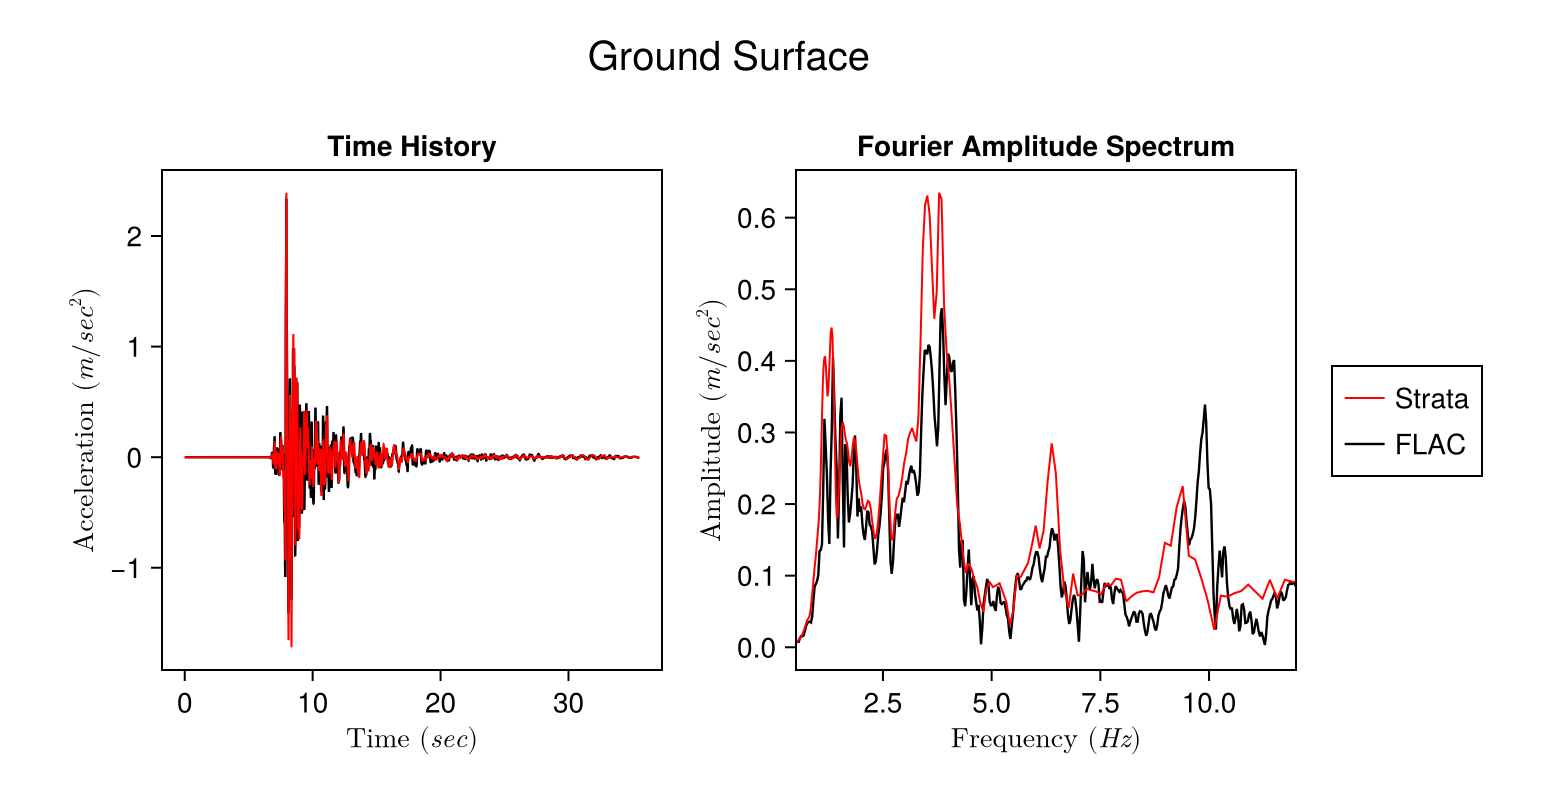
\includegraphics[width=\linewidth]{figures/fragility/Top-Non-Linear.png}
	\caption{Επιφανειακή Απόκριση Μη-Γραμμικής Ανάλυσης}
	\label{fig:nl-sur}
\end{figure}

Η προκύπτουσα απόκριση αποτυπώνεται στο Σχήμα \ref{fig:nl-sur}, όπου στην επιφάνεια είναι σαφές από την καταγραφή ότι τα πλάτη και το συχνοτικό περιεχόμενο έχουν πλέον εμφανείς διαφορές. Η απόκλιση στα πλάτη και τις συχνότητες προκύπτει σίγουρα και από το ισοδύναμο-ελαστικό μοντέλο, όπου επιλέγοντας μία μέση δυστμησία και απόσβεση, οι ισχυρές εδαφικές κινήσεις το έδαφος εμφανίζει χαμηλή απόσβεση και μεγάλη στιβαρότητα ενώ στις χαλαρές κινήσεις θα έχει πολύ υψηλή απόσβεση και ευκαμψία. Αυτό διαγράφεται καθαρά στο γεγονός ότι το Strata έχει μικρότερα πλάτα σε σχέση με του FLAC στις ανίσχυρες κινήσεις και μεγαλύτερα πλάτη στις ισχυρές. Πάντοτε αυτή η αναφορά έχει αξία, επιδιώκοντας τα αποτελέσματα του FLAC ως τα ακριβέστερα για το φυσικό πρόβλημα, και το Strata ως βοηθητικό εργαλείο επιβεβαίωσης.

Πιο αναλυτικά μπορεί να παρατηρηθεί το φάσμα πλάτους, του οποίου η μορφή έχει μία σχετικά καλή σύγκλιση στις πρώτες δύο συχνότητες συντονισμού, με εξαίρεση τα πλάτη, ενώ στις επόμενες δύο το συχνοτικό περιεχόμενο αρχίζει να συμπεριφέρεται διαφορετικά.

Στο Σχήμα \ref{fig:nl-tf} απεικονίζονται οι συναρτήσεις μεταφοράς. Η πρώτη συχνότητα συντονισμού συγκλίνει στα δύο εργαλεία και στην θεωρητική τιμή, καθώς και τα πλάτη της είναι ικανοποιητικά. Η δεύτερη και η τρίτη είναι επίσης αρκετά κοντά στα δύο εργαλεία, με εξαίρεση ότι η τρίτη έχει μεγάλη ενίσχυση στο αριθμητικό προσομοίωμα. Τέλος η τέταρτη συχνότητα εμφανίζει σπουδαία μείωση στο Strata σε σύγκριση με τις θεωρητικές, ενώ του FLAC είναι εγγύτερα. Το πλάτος είναι πάλι πολύ διαφορετικό στα δύο εργαλεία.

\begin{figure}[h]
	\centering
	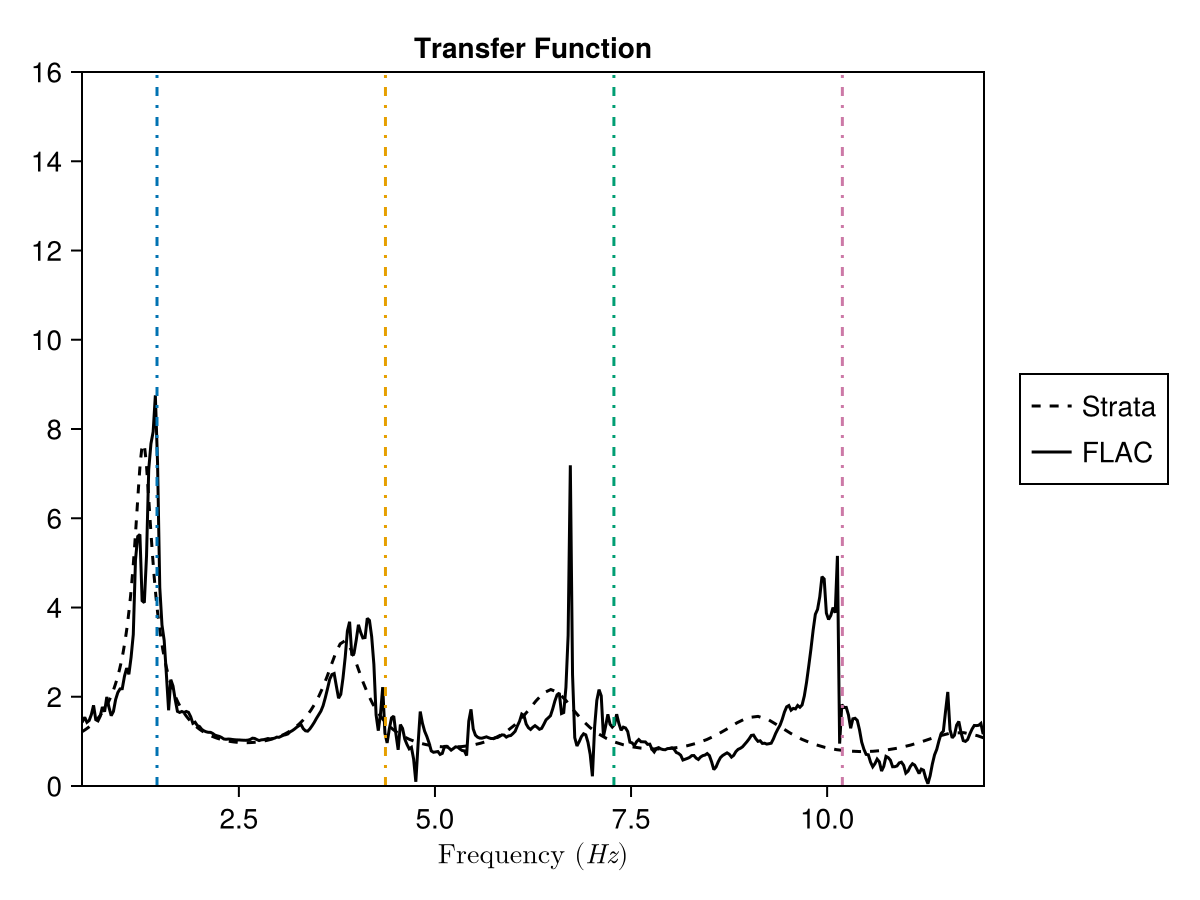
\includegraphics[width=0.8\linewidth]{figures/fragility/TF-Non-Linear.png}
	\caption{Συνάρτηση Μεταφοράς Μη-Γραμμικής Ανάλυσης}
	\label{fig:nl-tf}
\end{figure}

Κάθε συχνότητα συντονισμού είναι μειωμένη σε σχέση με τις θεωρητικές επιδεικνύοντας την αναφορά που έγινε σε προηγούμενη ενότητα, ότι δηλαδή η υστερητική απόσβεση προκαλεί μείωση στις συχνότητες συντονισμού.

Προς το παρόν η σύγκλιση των αποτελεσμάτων είναι ικανοποιητική, καθώς είναι αδύνατον ένα μη-γραμμικό μοντέλο να ταυτιστεί σε αποτελέσματα με το γραμμικό.

\subsection{Στρωματοποιημένο Προσομοίωμα}
Σε συνέχεια της βαθμονόμηση προσομοιώματος σύνθετης στρωματογραφίας, επιλέγεται να προσομοιωθεί μία ισοδύναμη στήλη εδαφική στήλη, η οποία να διαθέτει μέση ταχύτητα μετάδοσης διατμητικών κυμάτων και δυστμησία ίση με της αρχικής στήλης, ενώ τα στρώματα θα είναι στιφρότερα σε σχέση με το βάθος ως μία τυπική παρατήρηση στο πεδίο.

Οι εδαφικές τομές που αναλύονται στην εργασία δεν είναι γνησίως κατά αυτόν τον τρόπο, και στην στρωματογραφία της Θεσσαλονίκης υπάρχει αντίστοιχη περίπτωση όπου βαθύτερο στρώμα εμφανίζεται σε χαλαρότερη κατάσταση. Ενώ, λοιπόν, μία τέτοια ανάλυση παρουσιάζει ενδιαφέρον ως προς την βαθμονόμηση, επιλέγεται η απλούστερη περίπτωση πως η δυσκαμψία αναλογεί με το βάθος.

\begin{figure}[h]
	\centering
	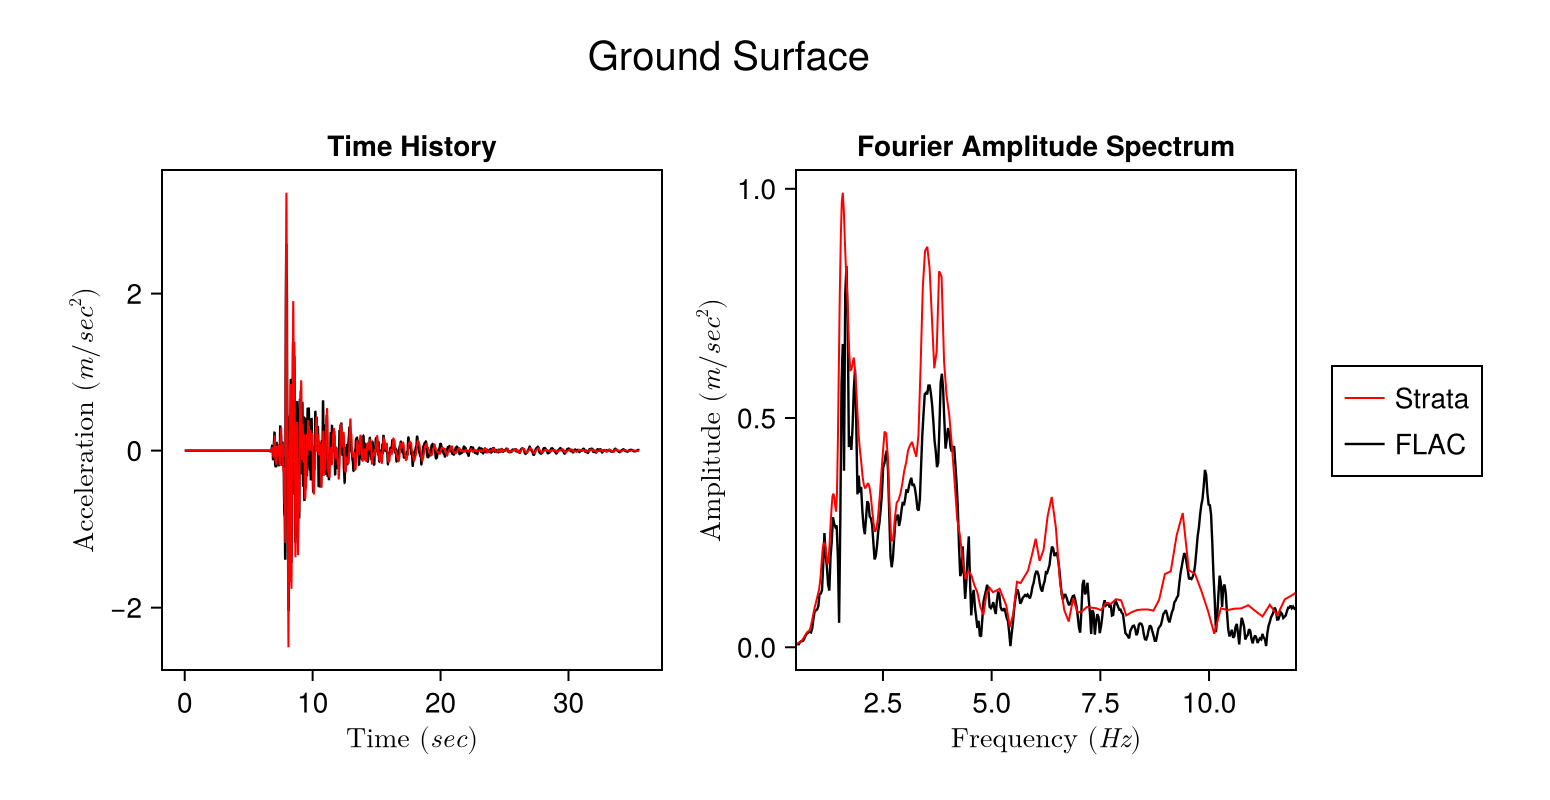
\includegraphics[width=\linewidth]{figures/fragility/Top-Stratified.png}
	\caption{Επιφανειακή Απόκριση Ελαστικής Στρωματοποιημένου Προσομοιώματος}
	\label{fig:str-sur}
\end{figure}

Το Σχήμα \ref{fig:str-sur} απεικονίζει την επιφανειακή απόκριση για το τελευταίο προσομοίωμα. Η καταγραφή φαίνεται να είναι παρόμοια με του μη-γραμμικού μοντέλου και όντως το φάσμα παρουσιάζει κοινή μορφή, με εξαίρεση ότι στην συγκεκριμένη περίπτωση η πρώτη συχνότητα συντονισμού έχει μεγαλύτερη απόκριση από τις υπόλοιπες.

Επίσης, το Strata διαθέτει δυνατότητα εισαγωγής στρωμάτων, επομένως το αντίστοιχο προσομοίωμα διαθέτει τα ίδια στρώματα ως προς την ταχύτητα $V_s$ και την υστερητική απόσβεση με το αριθμητικό προσομοίωμα, ενώ η ισοδύναμο γραμμική μέθοδος υπολογίζει αντιπροσοπευτικές τιμές δυστμησίας και απόσβεσης για κάθε στρώση ξεχωριστά.

\begin{figure}[h]
	\centering
	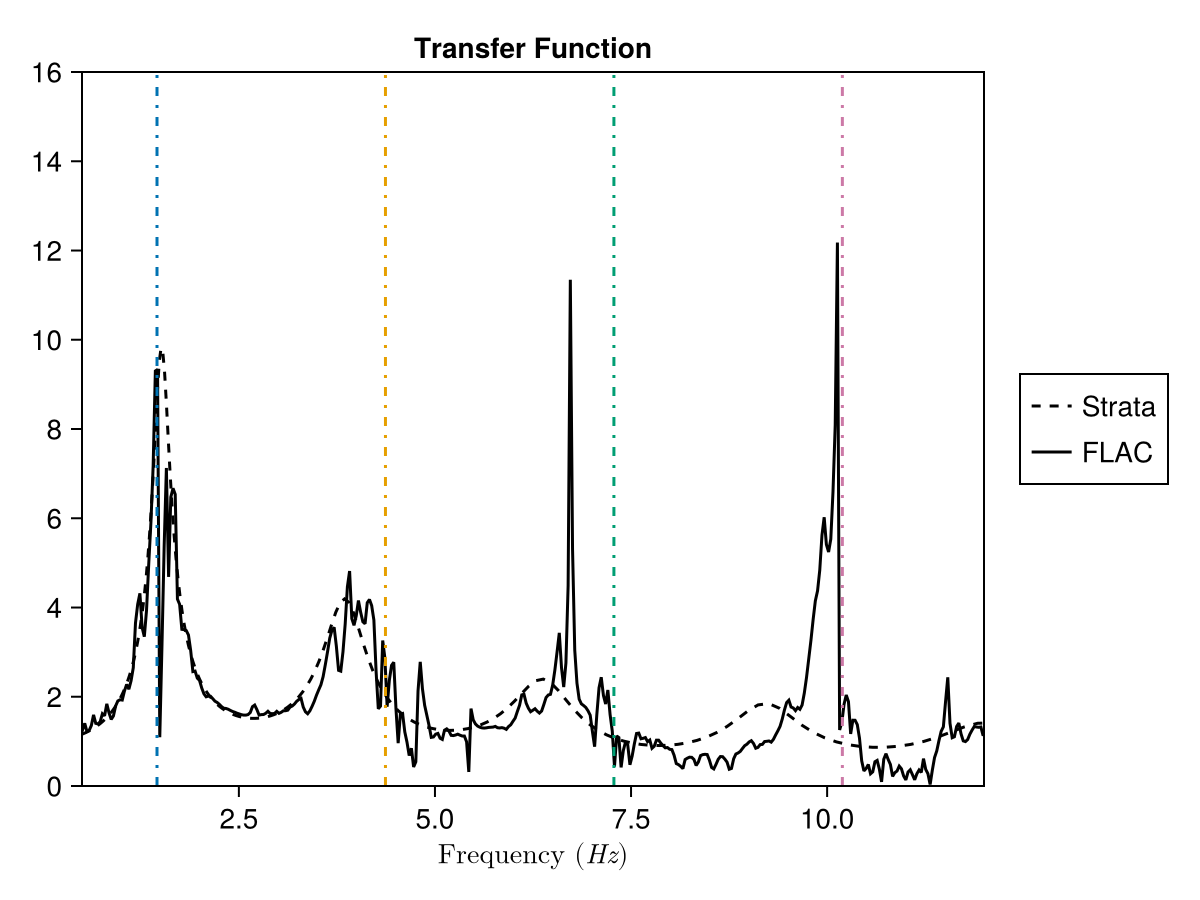
\includegraphics[width=0.8\linewidth]{figures/fragility/TF-Stratified.png}
	\caption{Συνάρτηση Μεταφοράς Στρωματοποιημένου Προσομοιώματος}
	\label{fig:str-tf}
\end{figure}

Από τα δύο φάσματα, υπολογίζεται η συνάρτηση μεταφοράς για την στρωματοποιημένη περίπτωση και αποτυπώνεται στο Σχήμα \ref{fig:str-tf}. Ο συντονισμός μοιάζει και στις δύο περιτπώσεις, υποννοώντας ευρυθμία και σε αυτό το προσομοίωμα, ενώ οι ενισχύσεις είναι αυξημένες.

\subsection{Συμπεράσματα Βαθμονόμησης}
Έχοντας ολοκληρώσει την βαθμονόμηση, και κρίνοντας εκ των αποτελεσμάτων, φαίνεται πως η αριθμητική προσομοίωση δυναμικών προβλημάτων προσεγγίζει ικανοποιητικά το φυσικό πρόβλημα.

Το συχνοτικό περιεχόμενο είναι κοντά στις προβλέψεις, ενώ η μικρή πτώση των συχνοτήτων συντονισμού στα υστερητικά μοντέλα είναι θετική ένδειξη.

Η βαθμός ενίσχυσης αντίστοιχα, παρουσιάζει εξαιρετική σύγκλιση για τις πρώτες δύο συχνότητες συντονισμού, οι οποίες είναι οι πιο προβλέψιμες συμπεριφορικά, προσφέροντας μία πολύ καλή συσχέτιση σε εύρος περιόδων $0.2-2\,sec$ που συνήθως αφορούν εδάφη κατηγορίας $C$ κατά Ευρωκώδικα.

Μία ενδιαφέρουσα διαφοροποίηση, της οποίας αιτία δεν επιτεύχθηκε διάγνωση, είναι η διακύμανση της ενίσχυσης μεταξύ των τριών προσομοιωμάτων. Η μεγαλύτερη ενίσχυση βρίσκεται φυσικά στο ελαστικό μοντέλο, για το οποίο δεν παρουσιάζεται υστερητική απόσβεση, έτσι ώστε να απορροφηθεί η σεισμική ενέργεια και να μειωθεί η απόκριση κατά την πλαστικοποίηση. Πρώτα όμως στο μονοστρωματικό προσομοίωμα η ενίσχυση μειώνεται σε σχέση με το ελαστικό, αλλά έπειτα στο πολυστρωματικό η ενίσχυση αυξάνεται και στην αριθμητική και στην ισοδύναμη-γραμμική μέθοδο.

Οι αιτίες που ένα τέτοιο φαινόμενο παρατηρείται μπορεί να είναι πολλές, καθώς ένα σεισμικό πρόβλημα είναι πολυπαραμετρικό και σύνθετο, και τέτοιες συμπεριφορές ενδέχεται να εμφανιστούν χωρίς να εντοπίζεται εύκολα η αιτία. Επομένως, αυτό αναφέρεται ως μία απλή παρατήρηση για την απρόβλεπτη συμπεριφορά των σεισμικών προβλημάτων, ενώ συγκρατείται μία λεπτή πιθανότητα να αποτελεί σφάλμα και να οφείλεται σε άγνωστη αλλά προσδιορίσιμη αιτία.

\section{Οριακές Καταστάσεις}
Έχοντας επιβεβαιώσει την λειτουργία των δυναμικών αναλύσεων, ίσως να ήταν το αναμενόμενο χωρικώς να ακολουθήσουν οι ίδιες οι δυναμικές αναλύσεις.

Τουναντίον, ο παρατηρητικός αναγνώστης θα διαπιστώσει πως δεν έχουν οριστεί ακόμα οι οριακές καταστάσεις λειτουργίας, γεγονός όπου θα μπορούσε να ακολουθεί τεχνικώς τις αναλύσεις, αλλά έχει και λογικώς.

Οι οριακές καταστάσεις επιλέγεται να είναι τρεις, ορίζοντας τις ως καταστάσεις μικρής, μέτριας και μεγάλης ζημίας.

Θεωρητικώς οι ορισμοί μοιάζουν αυθαίρετοι, αλλά, όπως θα φανεί και στην συνέχεια, ο αριθμητικός προσδιορισμός των οριακών καταστάσεων αστοχίας είναι απολύτως ορισμένος.

Η αστοχία της σήραγγας, θεωρείται όταν η δομή της κατασκευής ζημιώνεται, με αποτέλεσμα να υπεισέρχεται σε κάποιο ποσοστό στην μη-γραμμική (πλαστική) περιοχή του ωπλισμένου σκυροδέματος. Αυτός ο ορισμός αποτρέπει την πλαστικοποίηση και υστερητική συμπεριφορά του περιβάλλοντος εδάφους να καθορίσει κάποια οριακή κατάσταση αστοχίας, παρά μόνο εμμέσως από το σκυρόδεμα.

Αντίστοιχα, οι δυναμικές αναλύσεις σε εδάφη, όπου περιλαμβάνουν την υστερητική συμπεριφορά των εδαφών είναι πολύ σύνθετα προβλήματα καθώς και υπολογιστικώς κοστοβόρα. Έτσι, συνηθίζεται σε σεισμικές αναλύσεις σηράγγων, τα τοιχώματα της σήραγγας να συμπεριφέρονται με ελαστικό καταστατικό μοντέλο, και όχι με το πιο ακριβές ελαστοπλαστικό. Αυτό έχει ως αποτέλεσμα η ροπή και η παραμόρφωση που εμφανίζεται στην σήραγγα να υπακούει σχεδόν αποκλειστικά στην συμπεριφορά του εδάφους, χωρίς πρόσθετα φαινόμενα.

Μία τέτοια επιλογή, εμφανίζει, αφενός, το πολύ μεγάλο πλεονέκτημα ότι μειώνεται ο υπολογιστικός χρόνος του προσομοιώματος, όπου σε τέτοια προβλήματα μπορεί να είναι κρίσιμη παράμετρος για την βιωσιμότητα τον αναλύσεων. Αφετέρου, εφόσον η επιλογή των οριακών καταστάσεων έχει γίνει ήδη, τότε τα δυναμικά προσομοιώματα μπορούν να χρησιμοποιηθούν καθαρά για την παραγωγή της εξέλιξης των μεγεθών ζημίας με τον χρόνο. Για αυτόν τον λόγο λοιπόν και προηγείται ο ορισμός των οριακών καταστάσεων από τις αριθμητικές αναλύσεις.

\subsection{Μέθοδος Υπολογισμού}
%Pushover
Ως προς τους τρόπους εξαγωγής οριακών καταστάσεων, έχει αναπτυχθεί και περιγραφεί μία μέθοδος που συσχετίζει το μέγεθος ζημίας με την μη-γραμμική συμπεριφορά των υλικών κατασκευής.

%πως είναι το pushover στα ελληνικά; το γράφει στον Τσόπρα
Η συγκεκριμένη μέθοδος αφορά στην στατική pushover ανάλυση σηράγγων \parencite{TsinidisLS, Tsinidisfrag}. Τέτοιου είδους αναλύσεις εκτελούνται τοποθετώντας μία εξαναγκασμένη διαφορική μετατόπιση σε κάποιο προσομοίωμα και παρακολουθώντας την μη-γραμμική συμπεριφορά αυτής.

Στις σήραγγες, η ασκείται μία τριγωνική μετατόπιση σε μία εδαφική τομή, η οποία έχει εγκιβωτισμένη μία σήραγγα, και παρακολουθείται η εξέλιξη της ανηγμένης διαμετρικής παραμόρφωσης της. Το προσομοίωμα εδράζεται σε αρθρώσεις, ενώ πλευρικώς και στην επιφάνεια δεσμεύεται μόνο από τον καταναγκασμό. Η μορφή του προσομοιώματος περιγράφεται πολύ καλά στο Σχήμα \ref{fig:push}.

\begin{figure}[h]
	\centering
	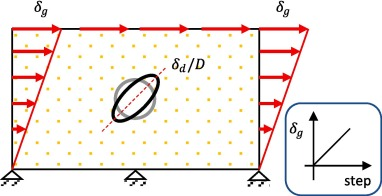
\includegraphics[width=0.7\linewidth]{figures/fragility/tsin-pushover.jpg}
	\caption{Αριθμητικό Προσομοίωμα Ανάλυσης Pushover \parencite{TsinidisLS}}
	\label{fig:push}
\end{figure}

Σε αυτού του είδους ανάλυση, το έδαφος προσομοιώνεται ως γραμμικώς ελαστικό, καθώς δεν ενδιαφέρει η πλαστικοποίηση και η παραμόρφωση του, ενώ τέτοια φαινόμενα θα προκαλούσαν αποσυντονισμό και υποεκτίμηση των επιδράσεων. Το σκυρόδεμα από την άλλη, πρέπει να μοντελοποιηθεί με πλήρη ελαστό-πλαστική συμπεριφορά, έτσι ώστε να αποφανθή η πραγματική του κατάσταση βλάβης.

Η ενέργεια τροπής της σήραγγας με την εξαναγκασμένη παραμόρφωση του εδάφους μπορεί να υπολογιστεί για κάθε βήμα παραμόρφωσης από την Εξίσωση \ref{eq:strain}. Η παραγώγιση της ενέργειας αυτής ως προς το EDP (την ανηγμένη διαμετρική παραμόρφωση), αποδίδει μία θεωρητική ισοδύναμη αξονική δύναμη $F_G$ στον δακτύλιο της σήραγγας, της ποίας η εξέλιξη αν παραγωγιστεί ξανά με το EDP παράγει την πορεία ελάττωσης της δυσκαμψίας $k_G$ με το EDP.

\begin{equation}
	U = \int \frac{1}{2} \sigma_{ij}\epsilon_{ij} dv
	\label{eq:strain}
\end{equation}

Σε σχέση με την αρχική δυσκαμψία $k_G0$, ορίζονται οι τρεις οριακές καταστάσεις από την γνωμάτευση ειδικών για τιμές του $k_G/k_{G0}$ ως 90\%, 75\% και 65\% αντίστοιχα για τις τρεις καταστάσεις που ορίστηκαν ήδη. Η πορεία υπολογισμού αποτυπώνεται στο Σχήμα \ref{fig:tsin-ls},

\begin{figure}[h]
	\centering
	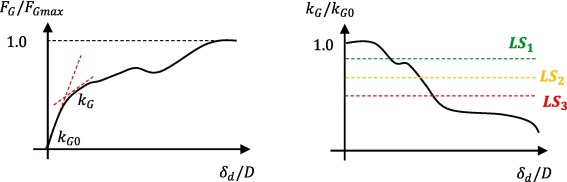
\includegraphics[width=0.7\linewidth]{figures/fragility/tsin-states.jpg}
	\caption{Ορισμός Οριακών Καταστάσεων \parencite{TsinidisLS}}
	\label{fig:tsin-ls}
\end{figure}

Οι οριακές καταστάσεις ορίστηκαν στην συγκεκριμένη μέθοδο για EDP την ανηγμένη διαμετρική παραμόρφωση, αλλά μία προσαρμογή της ανάλυσης θα μπορούσε πιθανότατα να πραγματοποιηθεί και για διαφορετικά EDPs.

\subsection{Ορισμός Ζημιωδών Καταστάσεων}
%Επιλογή από Τσινίδη
Η εκτέλεση των αναλύσεων pushover, ενώ είναι πραγματοποιήσιμη, θεωρήθηκε εν μέρη ότι ξεπερνάει τον σκοπό της παρούσας εργασίας, και δεν εκτελέστηκαν εξειδικευμένες αναλύσεις για τις εδαφικές τομές που επιλέχθηκαν.

Οι οριακές καταστάσεις όμως επιλέχθηκαν από την ενδελεχή εργασία των \cite{TsinidisLS}, και η μεθοδολογία θεωρήθηκε εξαιρετικά ενδιαφέρουσα για να μην αναπτυχθεί σε περιορισμένο βαθμό και εδώ.

Επίσης, έχει αναφερθεί ότι παράγονται καμπύλες τρωτότητας και για ροπές. Με EDP την ανηγμένη ροπή της διατομής στις $\pm 45 ^o$, οι οριακές καταστάσεις ορίζονται από τον Πίνακα \ref{tab:μ} \parencite{Huang}.

\begin{table}[]
	\begin{tabular}{lccccc}
		\hline
		\begin{tabular}[c]{@{}l@{}}Damage State\\ ($ds_i$)\end{tabular} & \begin{tabular}[c]{@{}c@{}}$ds_0$,\\ no damage\end{tabular}          & \begin{tabular}[c]{@{}c@{}}$ds_1$,\\ minor damage\end{tabular}             & \begin{tabular}[c]{@{}c@{}}$ds_2$,\\ moderate damage\end{tabular}          & \begin{tabular}[c]{@{}c@{}}$ds_3$,\\ extensive damage\end{tabular}        & \begin{tabular}[c]{@{}c@{}}$ds_4$,\\ collapse\end{tabular}           \\ \hline
		Range of DM                                                     & \begin{tabular}[c]{@{}c@{}}$M_{sd}/M_{Rd}$\\ $\leq 1.0$\end{tabular} & \begin{tabular}[c]{@{}c@{}}$ 1.0 <M_{sd}/M_{Rd}$\\ $\leq 1.5$\end{tabular} & \begin{tabular}[c]{@{}c@{}}$1.5 < M_{sd}/M_{Rd}$\\ $\leq 2.5$\end{tabular} & \begin{tabular}[c]{@{}c@{}}$2.5 <M_{sd}/M_{Rd}$\\ $\leq 3.5$\end{tabular} & \begin{tabular}[c]{@{}c@{}}$M_{sd}/M_{Rd}$\\ $\geq 3.5$\end{tabular} \\
		CCentral DM                                                     & -                                                                    & 1.25                                                                       & 2.00                                                                       & 3.00                                                                      & -                                                                    \\ \hline
	\end{tabular}
	\caption{Οριακές Καταστάσεις Ανηγμένων Ροπών}
	\label{tab:μ}
\end{table}

\section{Επιλογή Θέσεων}
% Πρέπει να βγάλω μηκοτομή, αλλιώς δεν γίνεται. Δεν θέλω να βάλω το autocad, δεν θα φαίνεται καλά, αν το χωρίσω σε τρία .pngs όμως δουλεύει.
%Η μηκοτομή χωρίζεται σε τρία τμήματα, αναφορά τα πλαίσια και μετά αναφορά στα υποτμήματα αυτών. Αφού χωριστούν τα τμήματα πρέπει να γίνει μία εκτενής αναφορά στα υλικά που τα συντελούν και τις ιδιότητες αυτών. Μάλλον σε αυτό το σημείο είναι το καλύτερο να βάλω την σύγκριση του vs30 και όχι στην διακινδύνευση.

Η πραγματοποίηση γεωτεχνικών μελετών και έργων είναι γνωστό ότι παρουσιάζει μία μόνιμη δυσκολία, ότι οι παράμετροι και οι συνθήκες παραμένουν άγνωστα μεγέθη στον μηχανικό.

Το έδαφος αποτελεί ένα χαρακτηριστικά ασυνεχές υλικό, όπου η δομή του δύναται να μεταβάλλεται σημαντικά ανά λίγα μέτρα ενώ οι γεωτεχνικές παράμετροι δεν γίνεται να προσδιοριστούν με απόλυτη ακρίβεια όταν ποικίλουν στον χώρο σε σχέση με την σύνθετη γεωλογία, τις τάσεις ή την υδρολογία.

Αυτή η περίπλοκη φύση είναι που θέτει τις κατάλληλες απλοποιήσεις και επιλογές ως εξαιρετικά κρίσιμες για την επιτυχία μίας μελέτης. Χωρίζοντας την απροσδιόριστη γεωλογία σε σαφή όρια που σχηματίζουν στρώματα, και επιλέγοντας αντιπροσωπευτικές τιμές των παραμέτρων, ένα γεωτεχνικό πρόβλημα μπορεί να προσομοιωθεί κατάλληλα ώστε να επιλυθεί.

Ακόμα περισσότερο σε ένα έργο μετρό, που εκτείνεται κατά μήκος μίας ολόκληρης πόλης, η γεωτεχνική έρευνα είναι βασικό στοιχείο της μελέτης και ιδιαίτερα της κατασκευής, αφού οι σήραγγες πρέπει να σχεδιάζονται με τέτοιον τρόπο ώστε να διανύουν τα κατάλληλα υλικά. Οι κατασκευαστικές ιδιότητες δεν ενδιαφέρουν εν προκειμένω, αλλά ενδιαφέρει η γεωτεχνική μηκοτομή της σήραγγας, από την οποία θα επιλεγούν τα σημεία δυναμικής μελέτης.

Κατά τον σχεδιασμό του μετρό Θεσσαλονίκης, εκτενείς γεωτεχνικές μελέτες πραγματοποιήθηκαν, προσδιορίζοντας πλήρως τα γεωλογικά, γεωτεχνικά και υδρολογικά χαρακτηριστικά του περιβάλλοντος του έργου εδάφους. Καθώς η τρισδιάστατη σεισμική ανάλυση αποτελεί δύσκολο εγχείρημα, για εργασίες άλλου βεληνεκούς, και η εκτέλεση αναλύσεων σε πυκνές εδαφικές τομές κατά μήκος του μετρό, η μόνη ρεαλιστική επιλογή είναι να αξιοποιηθούν αυτές οι μελέτες έτσι ώστε να κατασκευαστούν μερικές χαρακτηριστικές εδαφικές τομές, οι οποίες εύκολα θα ανάγονται στο σύνολο του έργου.

%Ακολούθως θα γίνει η αναφορά στην μηκοτομή, θα την φτιάξω αλλά είναι χαμαλοδουλειά και θα το κάνω μετά, μαζί και με καλύτερα Σχήματα τομών που να περιγράφουν καλά τις καταστάσεις.
Από την μελέτη, η μηκοτομή του μετρό χωρίζεται σε τρία τμήματα σύμφωνα με τα γεωτεχνικά χαρακτηριστικά τους, τα οποία με την σειρά τους χωρίζονται σε άλλα τρία, τρία και ένα υποτμήματα αντίστοιχα. Τα τμήματα αυτά εκτείνονται από τον Νέο Σιδηροδρομικό Σταθμό έως μετά το Πανεπιστήμιο, από πριν την Παπάφη έως την Βούλγαρη, και από την Βούλγαρη ως το Αμαξοστάσιο.

Τα εδάφη, οι γεωτεχνικές παράμετροι, τα πάχη των στρώσεων και η ερυθρά της σήραγγας διαφέρουν κατά μήκος του έργου αρκετά, και ο ακριβής χαρακτηρισμός του συνόλου με λίγες τομές είναι αδύνατον. Επομένως, η επιλογή των Χιλιομετρικών Θέσεων γίνεται καθαρά με σκοπό να ευρεθούν κάποια μέσα χαρακτηριστικά, των οποίων η εξαγωγή σε άλλες θέσεις να επιτρέπει μία ολιστική προσέγγιση στην τρωτότητα. Εξάλλου έννιαιες όπως η σεισμική τρωτότητα, συνήθως προσεγγίζονται με απλοποιητικές μεθόδους και η στατιστική επεξεργασία της επιτρέπει να φανεί χρήσιμη.

Τα υλικά που συντελούν την μηκοτομή ανήκουν σε τέσσερις κατηγορίες. Πρώτα από όλα σε μία μεγάλη έκταση, στο ιστορικό κέντρο της πόλης, υπάρχουν στην επιφάνεια του εδάφους ανθρωπογενείς αποθέσεις, παχών $2-10\;m$, οι οποίες ανταποκρίνονται στην οικιστική εξέλιξη της πόλης ανά τους αιώνες. Τα υλικά της στρώσης συμπεριφέρονται παρόμοια με χαλαρούς αμμοχάλικες.

Έπειτα, υπάρχει η Ενότητα Α1, η οποία αποτελείται από τεταρτογενείς αποθέσεις και χωρίζεται σε τρεις Υποενότητες. Το υλικό αυτό έχει παρόμοιες ιδιότητες με μαλακές αργίλους και συναντάται κατά βάση επιφανειακά στην μηκοτομή.

Η επόμενη Ενότητα είναι η Α2 που αποτελείται από τις πλέον χαρακτηριστικές, για την Θεσσαλονίκη, εδαφικές στρώσεις των καστανέρυθρων αργίλων. Οι καστανέρυθρες άργιλοι είναι γενικά πολύ στιφρές και σαν υλικό παρουσιάζουν υψηλές τιμές αστράγγιστης διατμητικής αντοχής.

Τέλος, σε κάποιες θέσεις εμφανίζεται η Ενότητα Β αποτελούμενη από ψαμμιτομάργες. Η συγκεκριμένη ενότητα είναι και αυτή αργιλική ενδιάμεσης δυστμησίας και αντοχής από τις άλλες δύο.

Από τις γεωτεχνικές μελέτες και τις εργαστηριακές δοκιμές των γεωτρήσεων, η πλαστιμότητα είναι παρόμοια σε όλες τις θέσεις, με την τιμή του δείκτη πλαστιμότητας να κυμαίνεται στα $PI = 10\%-30\%$. Η πλαστιμότητα των εδαφών είναι απαραίτητη για τον ορισμό καμπυλών G-γ-D.


%Εδώ θα γίνουν αναφορές στις τρεις μηκοτομές.
Αναλύοντας την κατανομή των εδαφικών στρώσεων, το πρώτο Τμήμα χωρίζεται σε τρία Υποτμήματα. Το Υποτμήμα 1 καλύπτει την απόσταση μεταξύ των χιλιομετρικών θέσεων 0-249.090 ως 0+443.00 και αποτελείται από τρία στρώματα των Ενοτήτων Α1 με πάχος περί των 25 μέτρων και μία επιφανειακή στρώση ανθρωπογενών αποθέσεων με πάχος γύρω στα 5 μέτρα. Η σήραγγα στο συγκεκριμένο Υποτμήμα εγκιβωτίζεται κυρίως σε υλικό Α1β.

Το Υποτμήμα 2 συνεχίζει έως την Χ.Θ. 1+908.00 αποτελούμενη κυρίως από υλικά κατηγορίας Α2 πάχους περί των 30 μέτρων και επικάλυψη ανθρωπογενών αποθέσεων που πλησιάζουν στις περισσότερες θέσεις τα 10 μέτρα. Σε θέσεις κοντά στον Σταθμό Δημοκρατίας, εμφανίζεται μία λεπτή στρώση από υλικό Α1 ενώ η σήραγγα εγκιβωτίζεται κυρίως σε υλικά Α2β και Α2γ.

Ολοκληρώνοντας το Τμήμα Α με το Υποτμήμα 3, φτάνοντας ως την Χ.Θ. 3+630.00, η δομή του είναι πολύ παρόμοια του Υποτμήματος 2, με διαφορά ότι δεν εμφανίζονται καθόλου υλικά Α1, και ότι η σήραγγα εγκιβωτίζεται σχεδόν κατά αποκλειστικότητα σε Α2γ.

Συνεχίζοντας με το Τμήμα Β, το αντίστοιχο Υποτμήμα 1 συνεχίζει έως την Χ.Θ. 4+250.00 με υπόβαθρο καστανέρυθρων αργίλων με υπερκείμενες στρώσεις από υλικά Β, Α1 και ανθρωπογενών αποθέσεων. Αυτό το μικρό Υποτμήμα λοιπόν πραγματοποιεί μία μετάβαση από τις καστανέρυθρες αργίλους σε μαργαϊκά υλικά.

Το Υποτμήμα 2 εκτείνεται έως την Χ.Θ. 5+800.00, με την σήραγγα να βρίσκεται εντός της υποκείμενης στρώσης Β μεγάλου πάχους 30 μέτρων με υπερκείμενες στρώσεις Α1 με συνολικό πάχος περί των 10 μέτρων.

Μέχρι την Χ.Θ. 7+120.00, το Υποτμήμα 3 αποτελείται από τρεις στρώσεις υλικών Ενότητας Α1 με την σήραγγα να είναι εγκιβωτισμένη σε Α1β και Α1γ υλικά. Η αλλαγή των Τμημάτων πραγματοποιείται ακριβώς πριν από τον Σταθμό της Βούλγαρη όπου συναντάται το ρήγμα της Βούλγαρη, αλλάζοντας απότομα την στρωματογραφία από υλικά Ενότητας Α1 σε υλικά Ενότητας Β.

Τελευταίο είναι το Τμήμα Γ που εκτείνεται έως το τέλος του έργου, στο αμαξοστάσιο της Πυλαίας, στην Χ.Θ. 9+656. Το Τμήμα είναι εννιαίο και αποτελείται σχεδόν αποκλειστικά από υλικά της Ενότητας Β ενώ σε ορισμένες θέσεις υπάρχουν επιφανειακές ανθρωπογενείς αποθέσεις και κάποιες πολύ λεπτές στρώσεις από την Ενότητα Α1.

Η ορθή προσομοίωση και ανάλυση του έργου θα έπρεπε να γίνει για κάθε Τμήμα και Υποτμήμα ξεχωριστά. Κάτι τέτοιο θα απαιτούσε σε ανάλυση τουλάχιστον οχτώ αναλύσεων, που σε συνδυασμό με τις 30 χρονοϊστορίες που θα επιλεγούν σε επόμενη Ενότητα της εργασίας, αυτό θα οδηγούσε στην εκτέλεση 210 δυναμικών αναλύσεων κατ' ελάχιστον. Η υπολογιστική δυνατότητα για εκτέλεση αναλύσεων είναι αρκετά περιορισμένη, έτσι επιλέγονται τρεις χαρακτηριστικές εδαφικές τομές, που να εμπεριέχουν όλες τις Ενότητες υλικών.

Έτσι, τα εφτά Υποτμήματα μοιράζονται σε τρεις χαρακτηριστικές τομές. Το Τμήμα Γ αντιστοιχεί σε μία μονοστρωματική εδαφική τομή από την Χ.Θ. 8+550 με την σήραγγα σε βάθος $14m$. Η επόμενη τομή κατασκευάστηκε από την Χ.Θ. 6+250 και αντιστοιχεί για τα μήκη του πρώτου Υποτμήματος του Τμήματος Α και για τα Υποτμήματα 2 και 3 του Τμήματος Β, η σήραγγα στην προκειμένη περίπτωση βρίσκεται σε βάθος 21 μέτρων και η τομή αποτελείται από τρεις στρώσεις Ενότητας Α1.

Τέλος από τα Υποτμημάτα 2 και 3 του Τμήματος Α και του Υποτμήματος 1 του Τμήματος Β, σχηματίζεται η εδαφική τομή Χ.Θ. 2+650, αποτελούμενη από δύο στρώσεις καστανέρυθρων αργίλων και υπερκείμενες ανθρωπογενείς αποθέσεις.

Αυτές οι τομές θα χρησιμοποιηθούν, και σε αυτό το σημείο είναι σημαντικό να αναφερθεί ότι τα διαφορετικά Υποτμήματα δεν διαφέρουν μονάχα στην στρωματογραφία, αλλά και στα εύρη παραμέτρων των ίδιων υλικών. Για αυτόν τον τρόπο η επιλογή τομών και υλικών γίνεται με σκοπό να παραχθεί μία μέση κατάσταση με όσο πιο απλά μέσα γίνεται, σε αντίθεση με την πλήρη αποτύπωση λεπτομερειών.

Πολλές συνθήκες επηρεάζουν τα τελικά αποτελέσματα των δυναμικών αναλύσεων, αλλά από αυτές διακρίνεται ως βασική η επιρροή της ταχύτητας μετάδοσης των διατμητικών κυμάτων $V_{S30}$ για την επιρροή των τοπικών εδαφικών συνθηκών και του λόγου ευκαμψίας, και του βάθους της σήραγγας για την παραμόρφωση της. Έτσι, συγκρίνονται οι τιμές αυτών των δύο παραμέτρων από την κατανομή των χαρακτηριστικών τομών με τις μετρηθείσες τιμές στο Σχήμα \ref{fig:char}.

\begin{figure}[h]
	\centering
	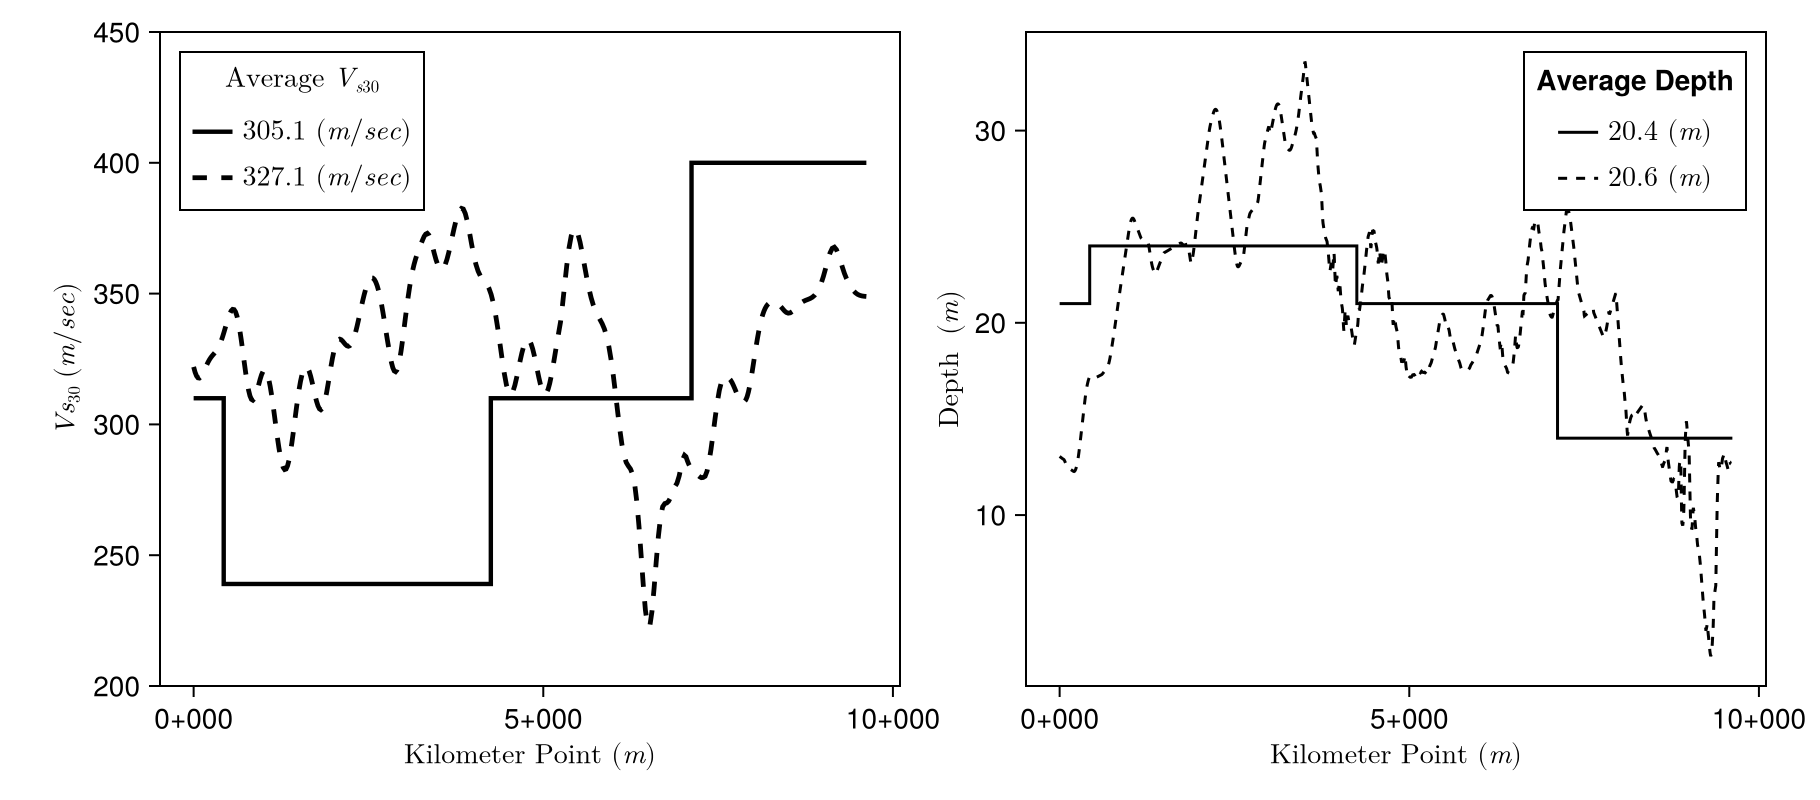
\includegraphics[width=1.03\linewidth]{figures/fragility/comparison.png}
	\caption{Σύγκριση Χαρακτηριστικών και Μετρηθέντων Τιμών}
	\label{fig:char}
\end{figure}

Το Σχήμα \ref{fig:char} παρουσιάζει μία αρκετά καλή, ποιοτική, σύγκριση στην περίπτωση των βαθών, όπου η ολική μέση τιμή είναι πολύ κοντά στην πραγματική μέση καθώς και οι μεμονωμένες χαρακτηριστικές τιμές, σε ένα σχετικό εύρος. Σε ορισμένες θέσεις βέβαια, η διακύμανση μεταξύ των βαθών φτάνει τα $5m-10m$, που είναι αρκετά από άποψη ποσότητας.

Πιθανό πρόβλημα στην κακή αντιπροσώπευση των εδαφών αφορά στον χαρακτηρισμό των σηράγγων. Η απόκριση μίας σήραγγας δεν αντιστοιχεί γραμμικά στο βάθος της, έτσι μία βαθύτερη ή επιφανειακότερη σήραγγα μπορεί να έχει εν γένει διαφορετική συμπεριφορά, επηρεάζοντας τόσο την παραμόρφωση της όσο τα μεγέθη έντασης και άλλες παραμέτρους. Έτσι, η άστοχη αναγωγή του βάθους μπορεί να επιφέρει απρόβλεπτα σφάλματα στον υπολογισμό της διακινδύνευσης.

Ως προς την μέση ταχύτητα, η μέση τιμή ανήκει στην ίδια τάξη μεγέθους, δίνοντας και την ίδια κατηγορία εδάφους ως C. Εμφανίζεται όμως πολύ μεγάλη διακύμανση στις ξεχωριστές τιμές, με σημαντική υποτίμηση της $V_{S30}$ στην δεύτερη και μεγάλη υπερτίμηση στην τρίτη χαρακτηριστική θέση.

Η μεγάλη απόκλιση στην ταχύτητα μπορεί να προκαλέσει διαφορετική συμπεριφορά στα διατμητικά κύματα, ενισχύοντας άλλες συχνότητες και προκαλώντας εντελώς διαφορετικές αποκρίσεις στην επιφάνεια και τις κατασκευές. Πιο συγκεκριμένα, η δεύτερη χαρακτηριστική θέση βρίσκεται σε μεγάλο βάθος σε στιφρές καστανέρυθρες αργίλους, επομένως η πρόκληση σημαντικών βλαβών θα αναμένονταν μόνο κατά την επιβολή πολύ ισχυρών χρονοϊστοριών.

Επί των αργίλων όμως, βρίσκεται μία παχιά στρώση από ανθρωπογενείς αποθέσεις, προσομοιωμένες ως χαλαροί χάλικες, της οποίας η χαμηλή διατμητική ταχύτητα επηρεάζει την μέση τιμή καθώς και τις τελικές επιφανειακές αποκρίσεις. Έτσι, η μέτρηση της έντασης που γίνεται στην επιφάνεια μπορεί να λαμβάνει μικρότερη τιμή της αναμενόμενης για συγκεκριμένες χρονοϊστορίες, ενώ η διαμετρική παραμόρφωση στην σήραγγα να είναι υψηλή, παρουσιάζοντας την συγκεκριμένη αίσθηση ως πιο τρωτή του αναμενόμενου. Εξάλλου η τιμή της $V_{S30}$ μπορεί να είναι αρκετά μεγαλύτερη σε πραγματικές συνθήκες, αλλά να υποτιμήθηκε το μέτρο δυστμησίας των ανθρωπογενών αποθέσεων.

Αντίστοιχα για την τρίτη χαρακτηριστική θέση, η υπερτίμηση της τιμής μπορεί να αλλοιώσει τα αποτελέσματα, θέτωντας την κατηγορία εδάφους της θέσης ως υψηλότερη.

Οι αποκλίσεις από την συμπεριφορά των εδαφών μπορούν να εξομαλυνθούν ελαφρώς σε τέτοιο εύρος από την εφαρμογή πληθώρας χρονοϊστοριών, μεγάλου εύρους σε ένταση και συχνοτικό περιεχόμενο. Οπότε, το φυσικό προσομοίωμα μπορεί να διαφέρει σημαντικά ενώ μία στατιστική προσέγγιση λιγότερο.

Φυσικά, οι μετρηθείσες τιμές της $V_{S30}$ προκύπτουν από τις γεωτρήσεις, ενώ η τιμές των χαρακτηριστικών θέσεων αναθέτοντας τιμές δυστμησίας στα εδάφη από τις γεωτρήσεις των μελετών. Επομένως, οι τιμές των εδαφικών τομών, που πραγματοποιήθηκαν συγκεκριμένα για το έργο είναι θεωρητικά ορθότερες από τις παρεμβολές γεωτρήσεων, αντιθέτως όμως, ενδέχεται οι τιμές των εργαστηριακών δοκιμών να εφαρμόσθηκαν λανθασμένα στο εύρος των θέσεων, δημιουργώντας την αποκλίνουσα εικόνα.

Οι αναλύσεις παρά όλα αυτά πραγματοποιούνται με τις τιμές των χαρακτηριστικών θέσεων, όποια και αν είναι η απόκλιση. Η εντύπωση του εύρος όμως είναι χρήσιμη για τα αποτελέσματα.

%\section{Βιβλιογραφικά Δεδομένα}

\section{Αναλύσεις}



\subsection{Γεωμετρία \& Υλικά}


%\subsection{Γεωτεχνικά Δεδομένα}



\section{Καμπύλες Τρωτότητας}
%Περιγραφή μεθόδου, εξιώσεις και τέτοια










\subsection{Πιθανοτικό Μοντέλο Σεισμικής Επάρκειας}
% Εξισώσεις
(PSDM, Probabilistic Seismic Demand Models)













